\begin{minipage}[H]{0.5\linewidth}
\section{MOEA/D. Experimentación y resultados}
\justify

La implementación del algoritmo propuesto se ha llevado a cabo utilizado el lenguaje \textit{Python} haciendo uso de las librerías \textit{Numpy}, para el manejo de vectores y matrices, \textit{os} y \textit{shutil} para el manejo de los ficheros y directorios, y \textit{matplotlib} y \textit{colour} para algunas representaciones gráficas. El código Python (débidamente comentado) se encuentra disponible en: \href{https://github.com/vicramgon/EV_BIII.git}{\color{blue} Código MOEA/D}. Para la evaluación de las métricas se ha utilizado el software proporcionado en la asignatura. \\

A continuación se muestran los resultados obtenidos para la evaluación del algoritmo propuesto con los distintos operadores. Para ello testearemos el mismo con la función matemática ZDT3 (con 30 dimensiones)\cite{zdt3}, comprobando tanto el comportamiento del mismo como evaluando una serie de métricas para los distintos operadores y comparándolo también con el algoritmo de referencia \textit{NSGA-II} \cite{Deb2002}.\\

\subsection{Evaluación MOEA/D + EOP1 con ZDT3}

Vamos a realizar algunas pruebas para comprobar la efectividad del algoritmo. Tanto utilizando una capacidad de cómputo de $10000$ evaluaciones (en distintos casos) como una de $4000$ evaluaciones (con distintos repartos). Para ello mostraremos algunas gráficas del comportamiento típico del algoritmo. Aunque en esta sección se muestra una o dos ejecuciones se han realizado 10 ejecuciones, cuyos resultados se presentan en los apéndices.\\


\end{minipage} \hfill
\begin{minipage}[H]{0.47\linewidth}
    \begin{figure}[H]
        \centering
        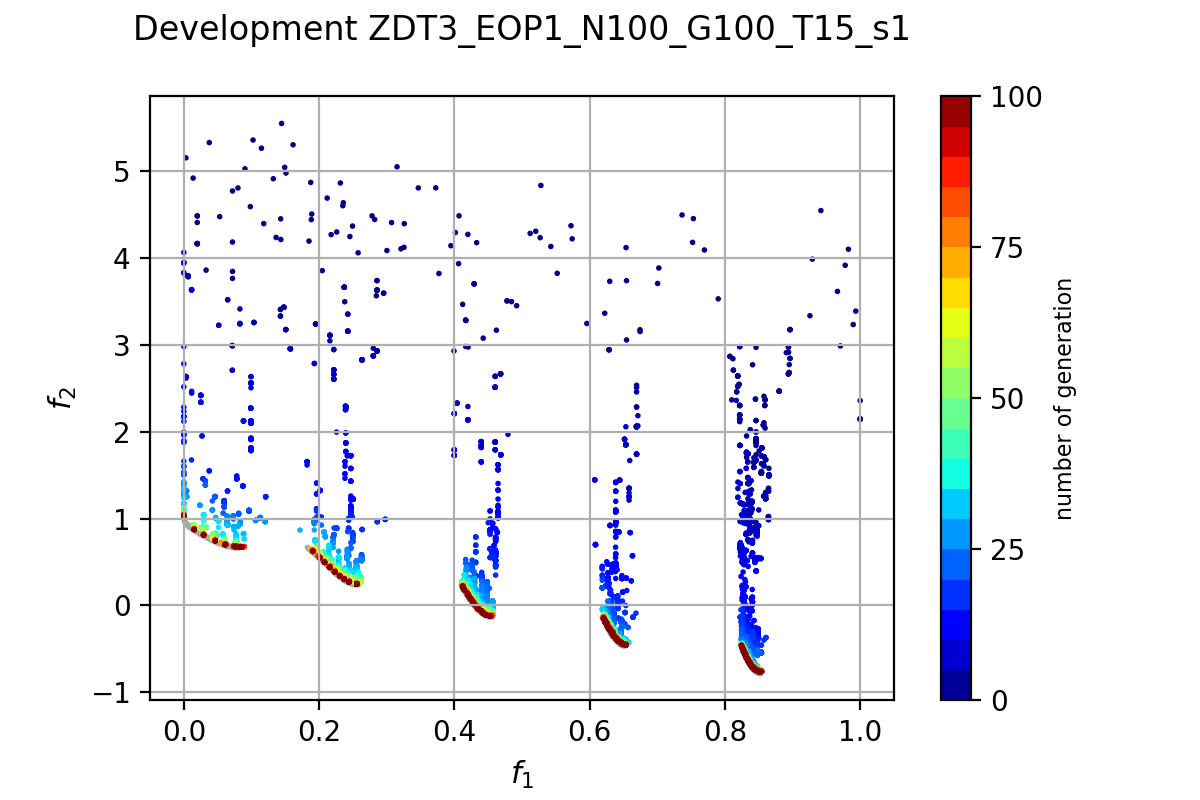
\includegraphics[scale=0.55]{figures/ZDT3_EOP1_N100_G100_T15/s1_dev.png}\\
        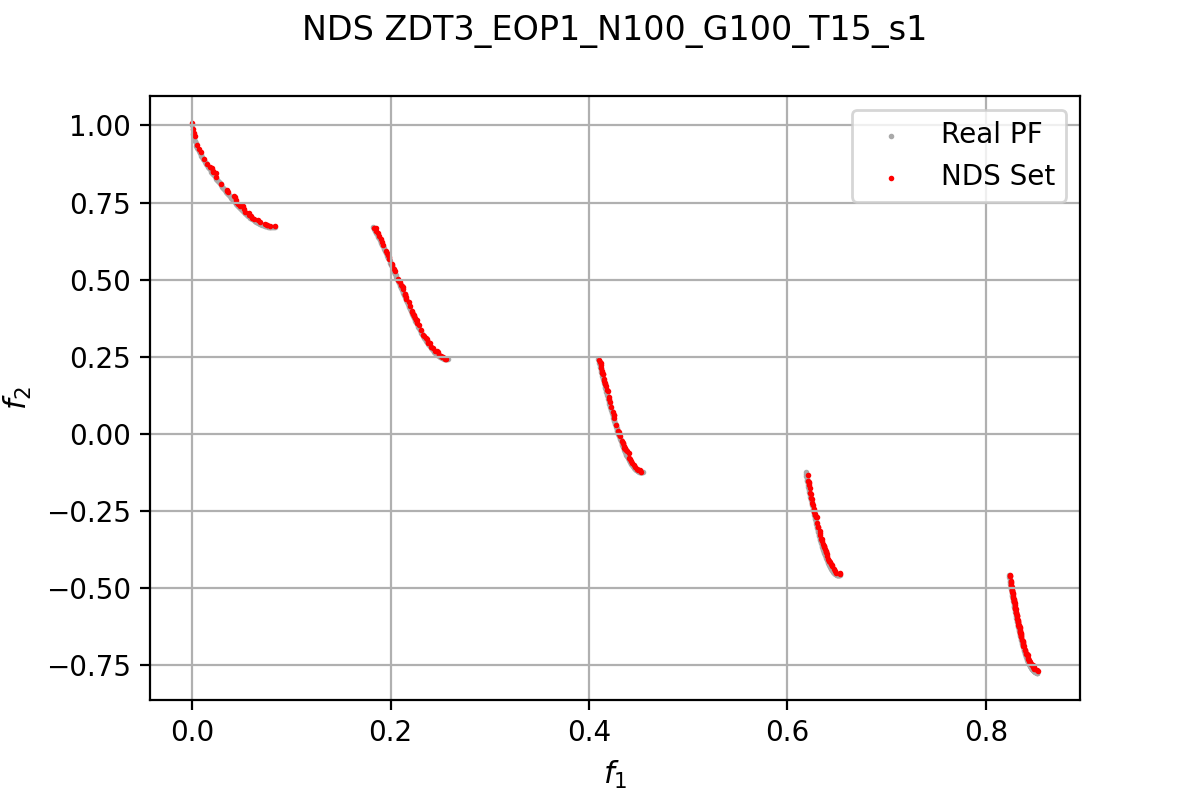
\includegraphics[scale=0.5]{figures/ZDT3_EOP1_N100_G100_T15/s1_nds.png}\\
        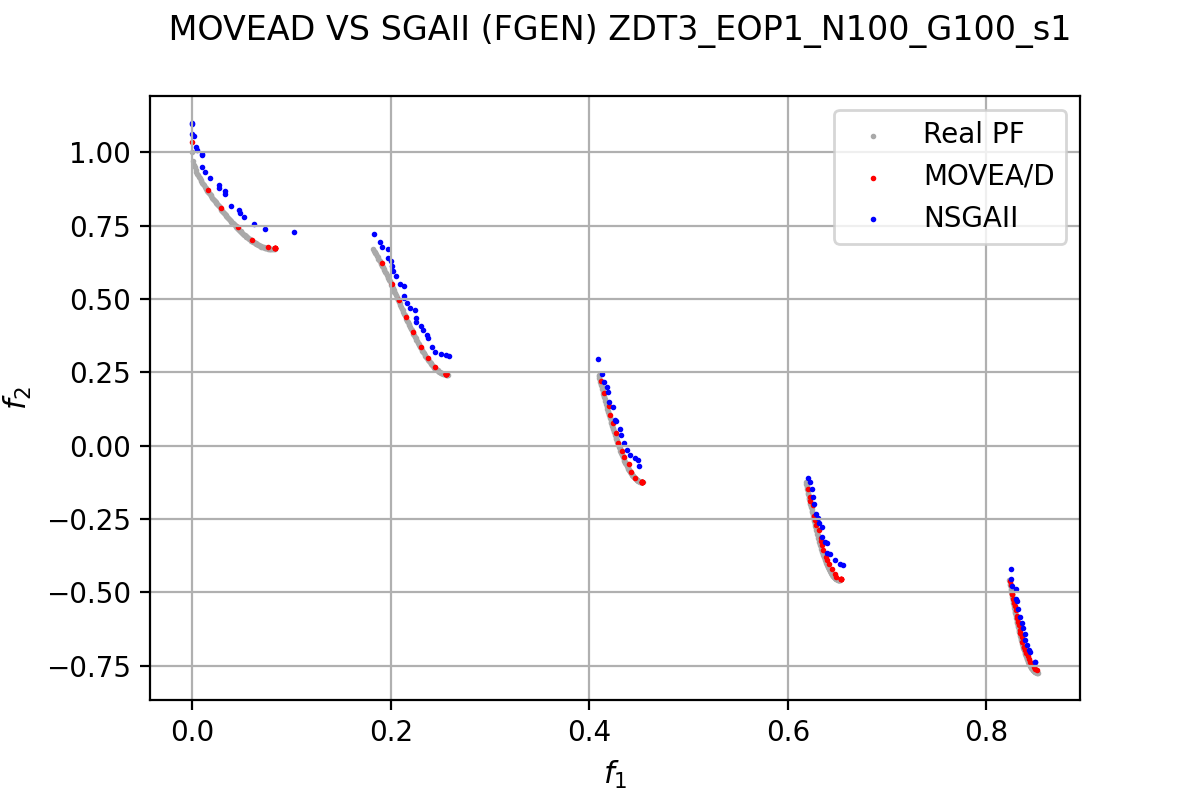
\includegraphics[scale=0.5]{figures/ZDT3_EOP1_N100_G100_T15/s1_comp.png}\\
        \caption{MOEA/D + EOP1 + N100G100}
        \label{fig:2}
    \end{figure}

    \vfill
    \end{minipage}\\

\justify
\subsubsection{Experimentación con 1OOOO ev.}

En este apartado realizamos un estudio (gráfico) del comportamiento del algoritmo, analizando la convergencia y diversidad de la población a lo largo de la ejecución del algoritmo. Propósito de tal estudio es además tratar de esclarecer la influencia de los parámetros $G$ y $N$ en el proceso evolutivo presentando una comparativa de las soluciones finales variando dichos parámetros, manteniendo constante el número de evaluaciontes, para los casos $(G=100, N=100)$, $(G=250, N=40)$ y $(G=50, N=200)$.\\

En la \hyperref[fig:2]{\textit{figura 2}} presentamos tres gráficos pertenecientes a una ejecución característica del algoritmo con el operador evolutivo EOP1, $N=100, G=100$ y $T=15$ (para todos los casos se ha tomado un $15\%$  (recuérdese que en los anexos se muestran varias ejecuciones que validan las discusiones) el primrer diagrama muestra el desarrollo de las soluciones en el espacio de objetivos a lo largo de la ejecución del algoritmo (en las distiontas generaciones). En él podemos apreciar que, tal como esperábamos a medida que el algoritmo avanza (pasan las generaciones) las soluciones tinden a ir convergiendo hacia el frente real de Pareto (señalado en gris), además de forma bastante rápida (los azules corresponden a las primeras generaciones y los anaranjados y rojos a las últimas) de forma que en menos de 50 generaciones se sitúan ya próximas al frente real. Otro aspecto a destacar es la diversidad, en los algoritmos evolutivos es corriente que las soluciones tiendan a concentrarse (se pierde diversidad); en este caso podemos ver dicha tendencia pero al mismo tiempo se puede notar que se tiende a conservar cierta dispersión en los puntos lo que denota una intención de mantener la diversidad (objetivo de todo algoritmo evolutivo).\\

En el segundo diagrama se presenta el conjunto de las soluciones no dominadas calculadas por el algoritmo, que parece corresponder en gran medida con el frente real de pareto, tanto en proximidad (convergencia) como en cobertura (dispersión) en los puntos del frente. Lo que denota, a priori, y a falta de métricas un buen comportamiento del algoritmo. De hecho, esos puntos podrían ser considerados como la salida del algoritmo, esto es la aproximación al frente de pareto que parece ser fiel al frente real (mostrado en gris).\\

Finalmente, presentamos una gráfica comparativa para nuestro algoritmo y para el algoritmo \textit{NSGA-II}. Para ello hemos representado las soluciones en el espacio de objetivos, las cuales corresponden a la última generación de ejecuciones en iguales condiciones $(G=100, N=100)$ para ambos algoritmos. Podemos ver que en cuanto a convergencia (proximidad al frente real) el frente del nuestro algoritmo es sensiblemente mejor que el frente proporcionado por  \textit{NSGA-II} (una gran mayoría de los puntos rojos están por debajo de los azules), mientras que en dispersión parece que los puntos del frente de \textit{NSGA-II} se distribuyen más uniformemente que los de nuestro algoritmo. Pero nótese que si consideramos como salida la proporcionada por el frente de las soluciones no dominadas la tanto la cobertura como la convergencia parecen más que aceptables.\\


Veámos ahora unas gráficas análogas a las presentadas pero para el caso $(G=250, N=40)$ en la \hyperref[fig:3]{\textit{figura 3}} podemos notar que el comportamiento es similar al caso anterior, esto es, como se espera a través de las generaciones las soluciones van aproximándose la convergencia al igual que en el caso anterior sigue siendo es buena, sin embargo se nota que la reducción en el número de subproblemas afecta de manera notable a la dispersión, sobre todo en las últimas generaciones. Sin embargo, si miramos el frente de soluciones no dominadas, vemos que tanto en convergencia (a priori, sin otro algoritmo de referencia) que tanto el grado de convergencia de las soluciones como el grado de dispersión hacen que se aproximen en buena medida al frente real de pareto, por lo que nos incita a pensar que la pérdida de diversidad debe darse relativamente al final porque existen soluciones buenas a lo largo prácticamente de todo el frente. Si comparamos ahora la última generación con la del algoritmo \textit{NSGA-II} (ejecutado en las mismas condiciones) podemos ver que ahora la superioridad no es tan patente como en el casi anterior y ambos algoritmos alcanzan un grado análogo de convergencia y dispersión (en este último aspecto quizá \textit{NSGA-II} parezca un poco mejor).\\

\begin{minipage}[H]{0.47\linewidth}
\begin{figure}[H]
        \centering
        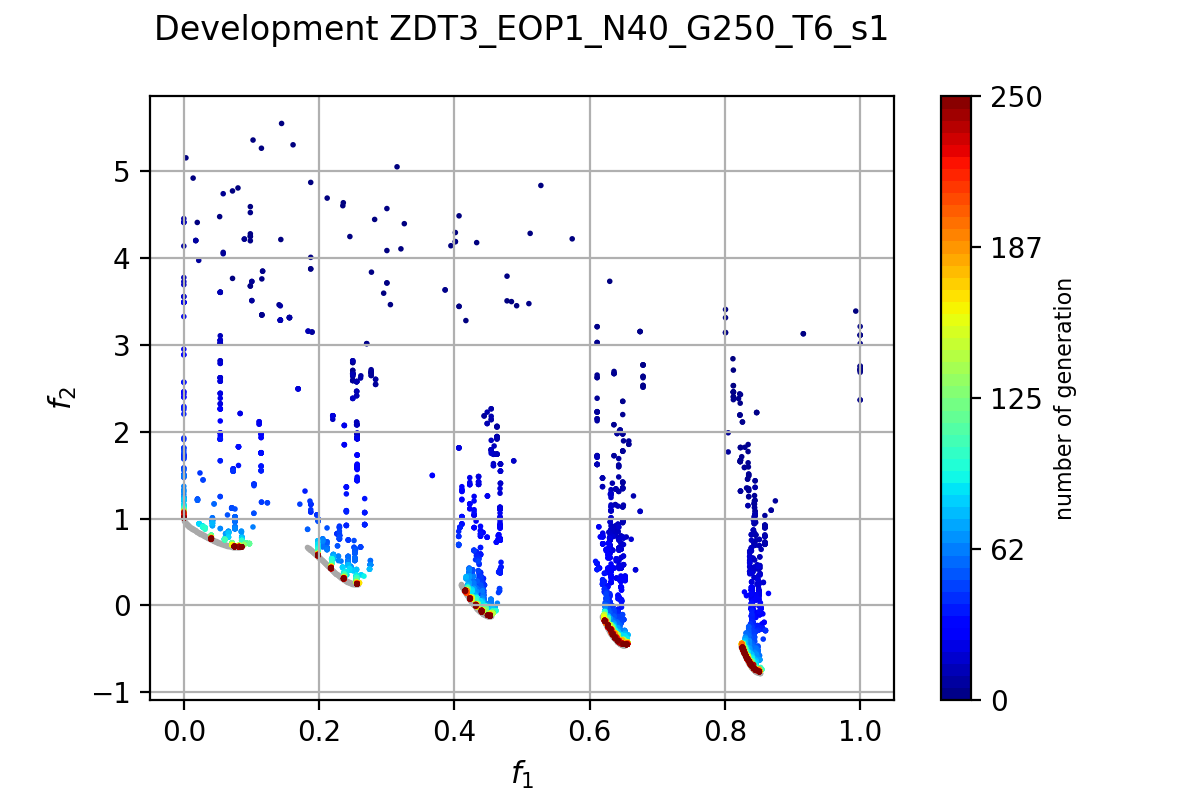
\includegraphics[scale=0.55]{figures/ZDT3_EOP1_N40_G250_T6/s1_dev.png}\\
        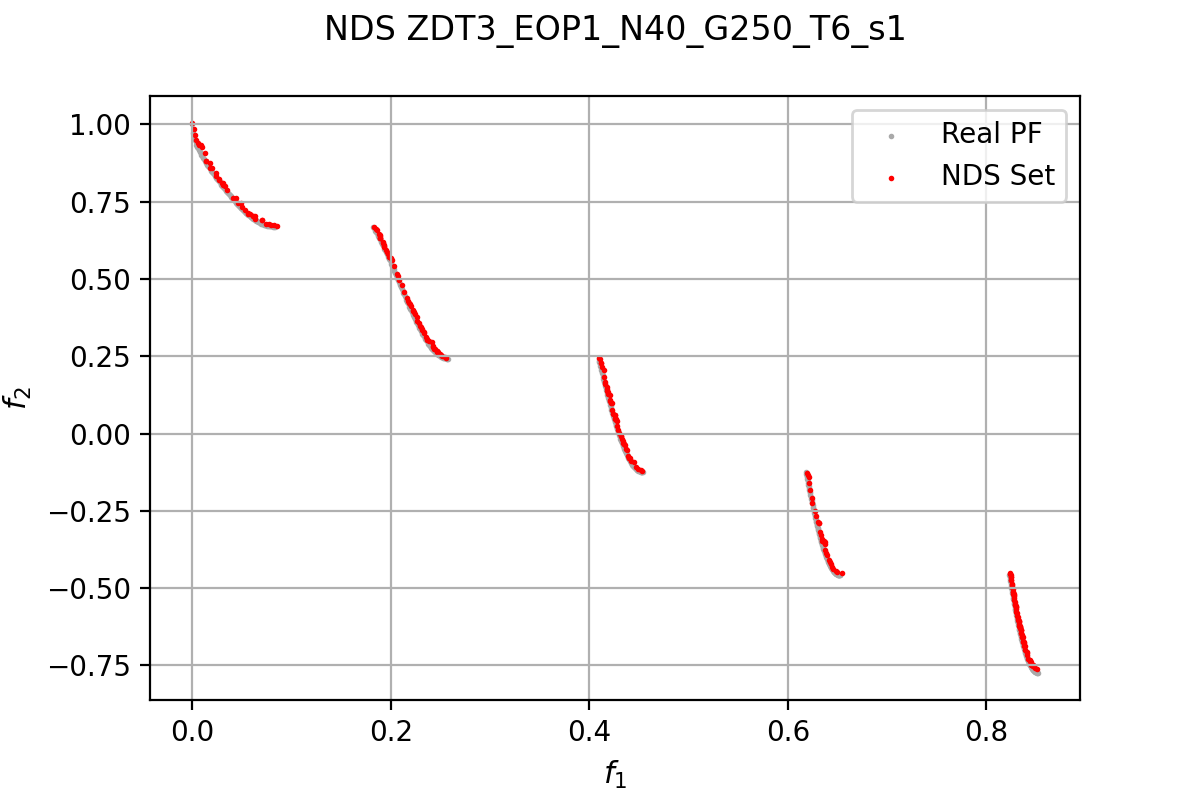
\includegraphics[scale=0.5]{figures/ZDT3_EOP1_N40_G250_T6/s1_nds.png}\\
        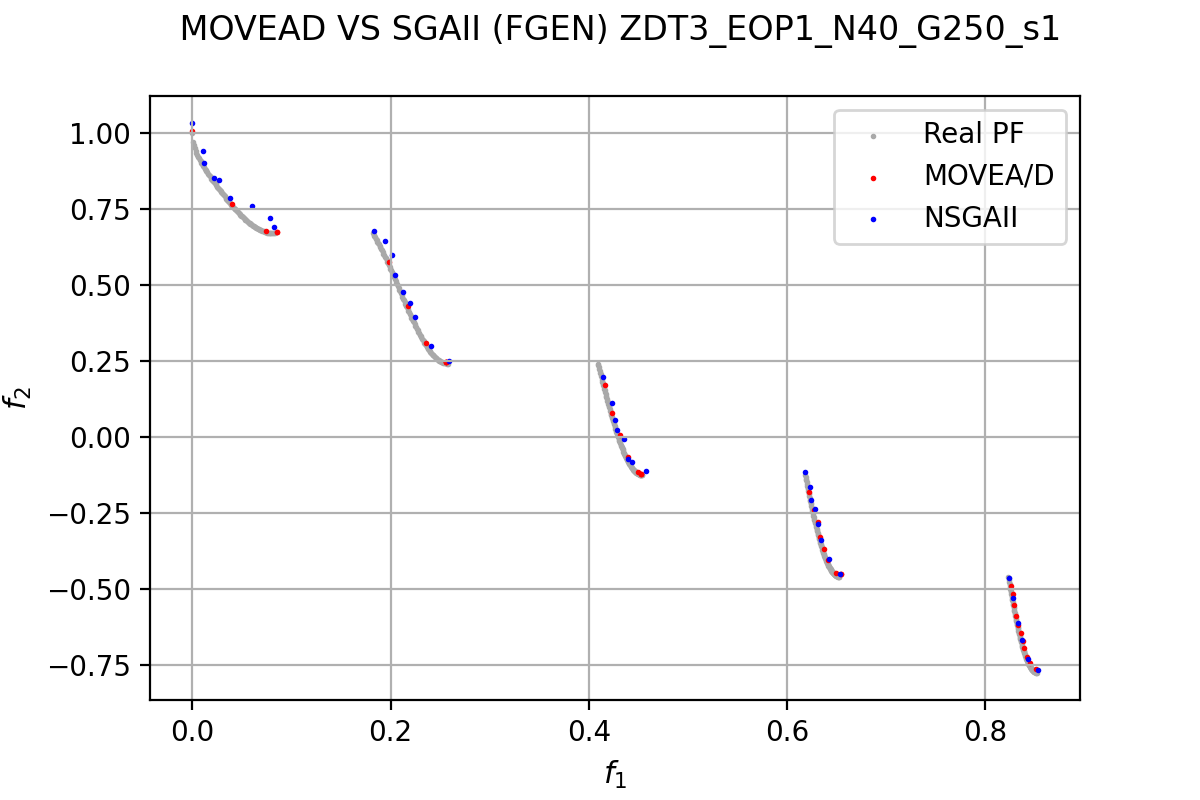
\includegraphics[scale=0.5]{figures/ZDT3_EOP1_N40_G250_T6/s1_comp.png}\\
        \caption{MOEA/D + EOP1 + N40G250}
        \label{fig:3}
    \end{figure}
\end{minipage} \hfill
\begin{minipage}[H]{0.47\linewidth}
    \begin{figure}[H]
        \centering
        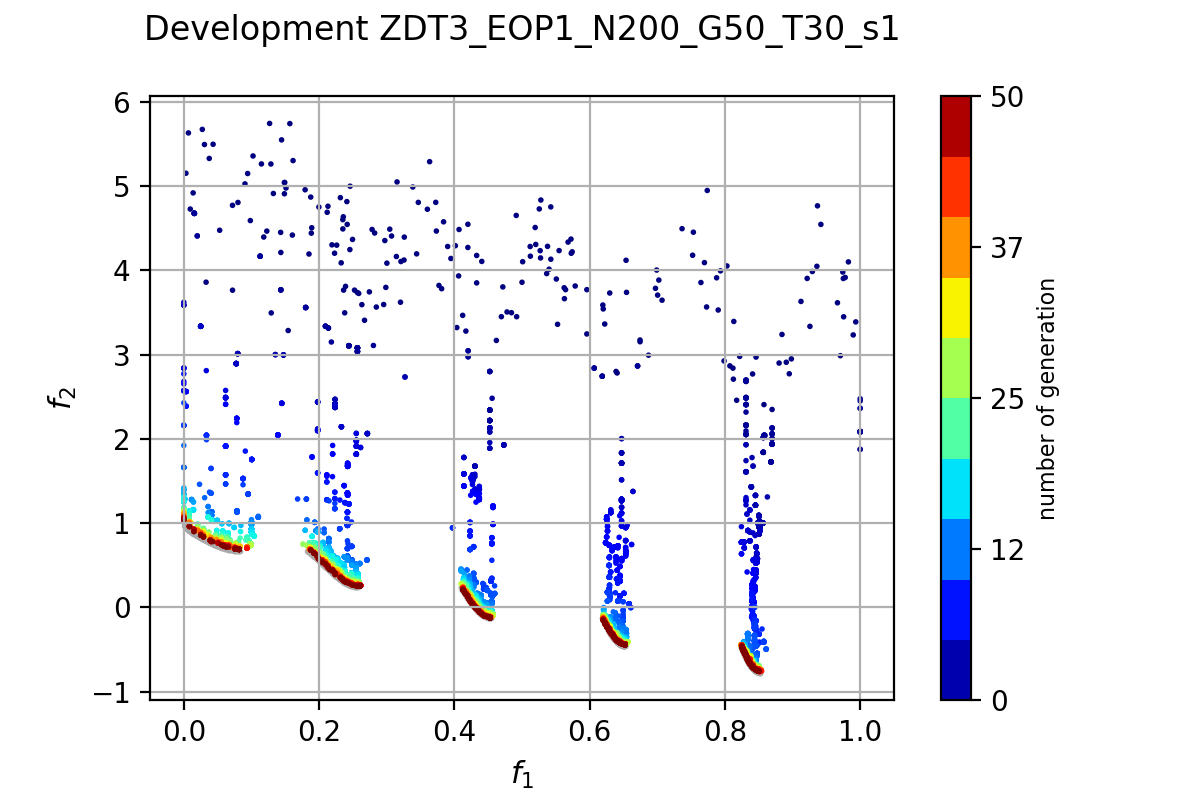
\includegraphics[scale=0.55]{figures/ZDT3_EOP1_N200_G50_T30/s1_dev.png}\\
        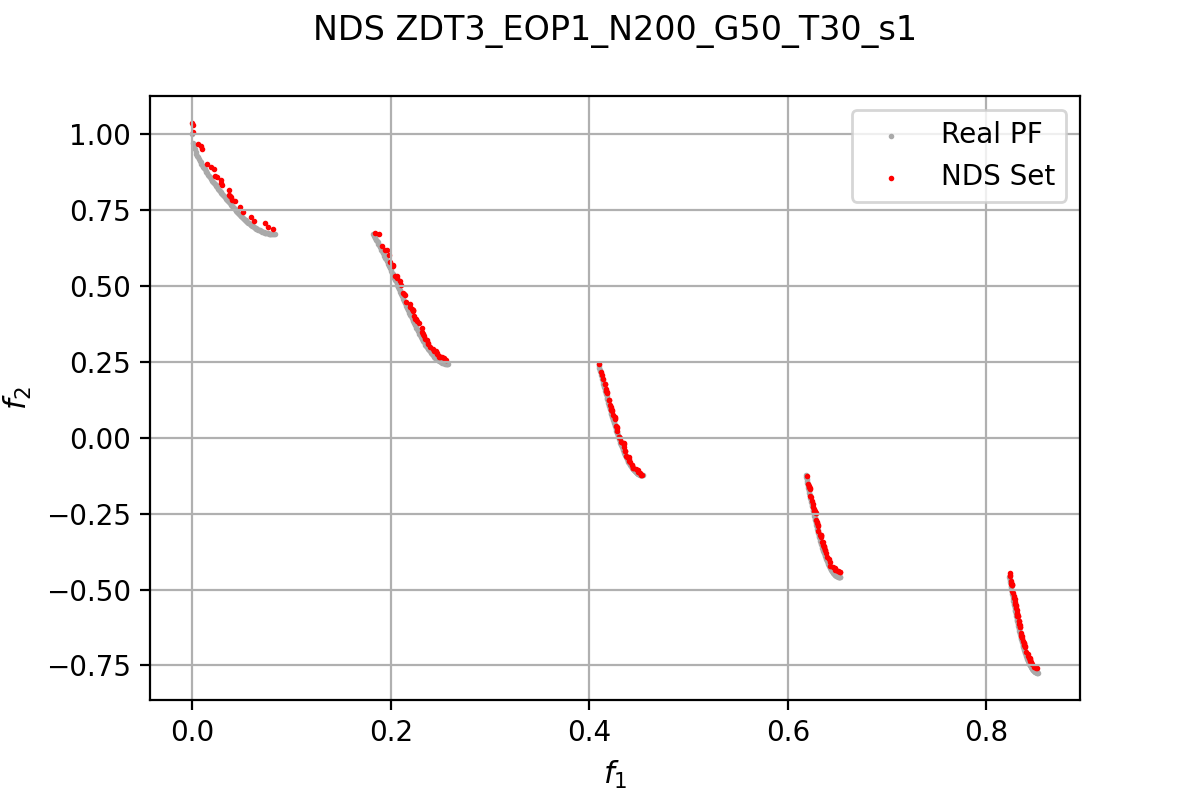
\includegraphics[scale=0.5]{figures/ZDT3_EOP1_N200_G50_T30/s1_nds.png}\\
        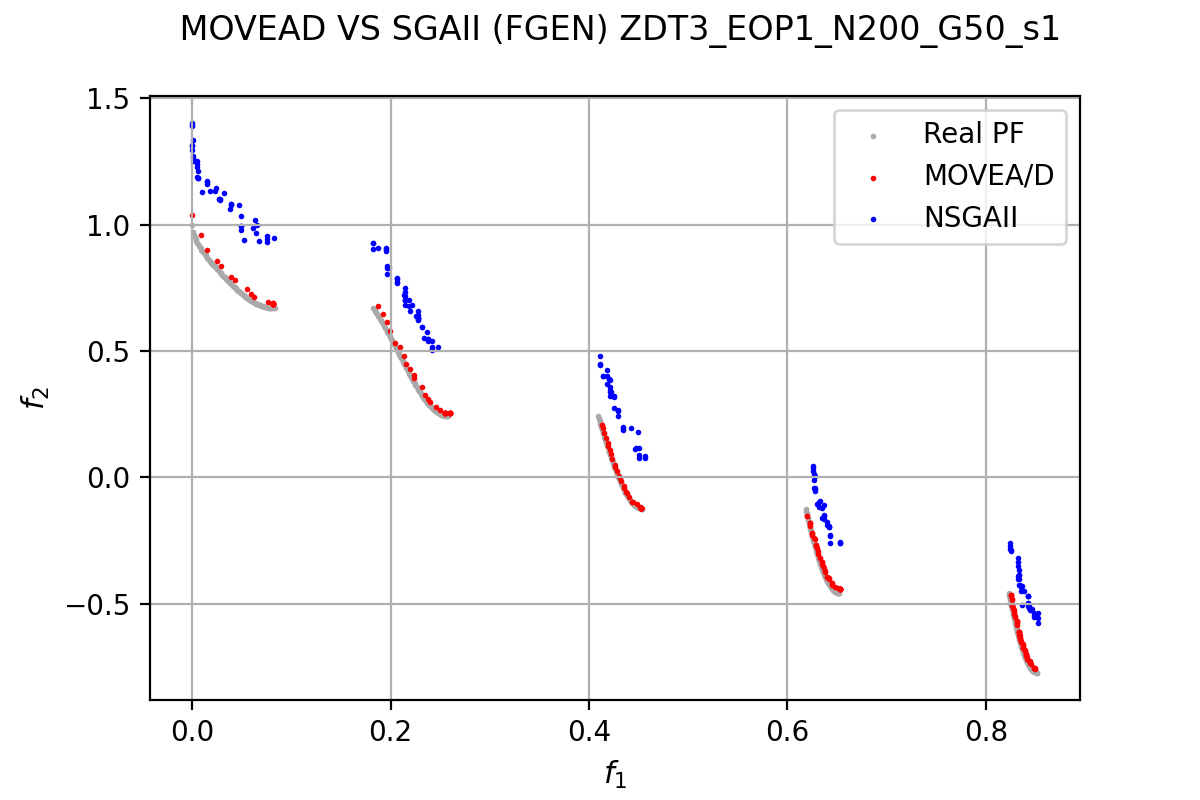
\includegraphics[scale=0.5]{figures/ZDT3_EOP1_N200_G50_T30/s1_comp.png}\\
        \caption{MOEA/D + EOP1 + N200G50}
        \label{fig:4}
    \end{figure}

    \vfill
    \end{minipage}\\


Y en último lugar comprobemos cuál es el resultado de elevar el número de subproblemas frente al número de generaciones. Dado que según hemos visto hasta ahora lo convergencia suele ser rápida, y que el número de subproblemas favorecerá la diversidad, a priori el comportamiento debería ser satisfactorio. Veámos qué ocurre para el caso $(G=250, N=40)$ en las gráficas presentadas en la \hyperref[fig:4]{\textit{figura 4}}. Podemos notar que la convergencia es bastante buena y la diversidad también permite que en las últimas generaciones se cubran los tramos del frente de manera más o menos uniforme. De hecho, si observamos el diagrama de las soluciones no dominadas podemos notar que, primero el ajuste es ligeramente peor que en los otros casos (normal dado que tiene menos generaciones para tratar de ajustarse) y la cobertura es buena y se reparte de forma más o menos uniforme. Si comparamos con la ejecución del \textit{NSGA-II} en este caso nuestro algoritmo es claramente mejor en convergencia y también algo mejor en cobertura (tramos más largos). \\

Finalmente vamos a realizar una comparativa entre los tres casos tanto para los frentes de la última generación como para los frentes \textit{NSD}. En la \hyperref[fig:5]{\textit{figura 5}} se muestran las dos gráficas de comparativa de los frente anteriormente indicados. En cuanto a las soluciones de la generación final todas se encuentran bastante superpuestas, quizá la roja con con una ligera menor convergencia (proximidad al frente) y la verde con una menor convergencia pudiendo ser la azul la más adecuada, esto es un balance en el número de generaciones y número de subproblemas lo que proporciona la mejor solución, aunque los resultados no son concluyentes y trataremos de realizar un estudio más profundo con el uso de las métricas. \\

En cuanto al NSD, las sensaciones son similares se nota bastante superposición entre los puntos, quizá con la roja un poco menor de convergencia en algunas partes y la azul y la verde muy similares, los resultados no son nada concluyentes, así que intentaremos clarificarlos con el uso de métricas y el correspondiente estudio estadístico de las mismas. 

\begin{center}
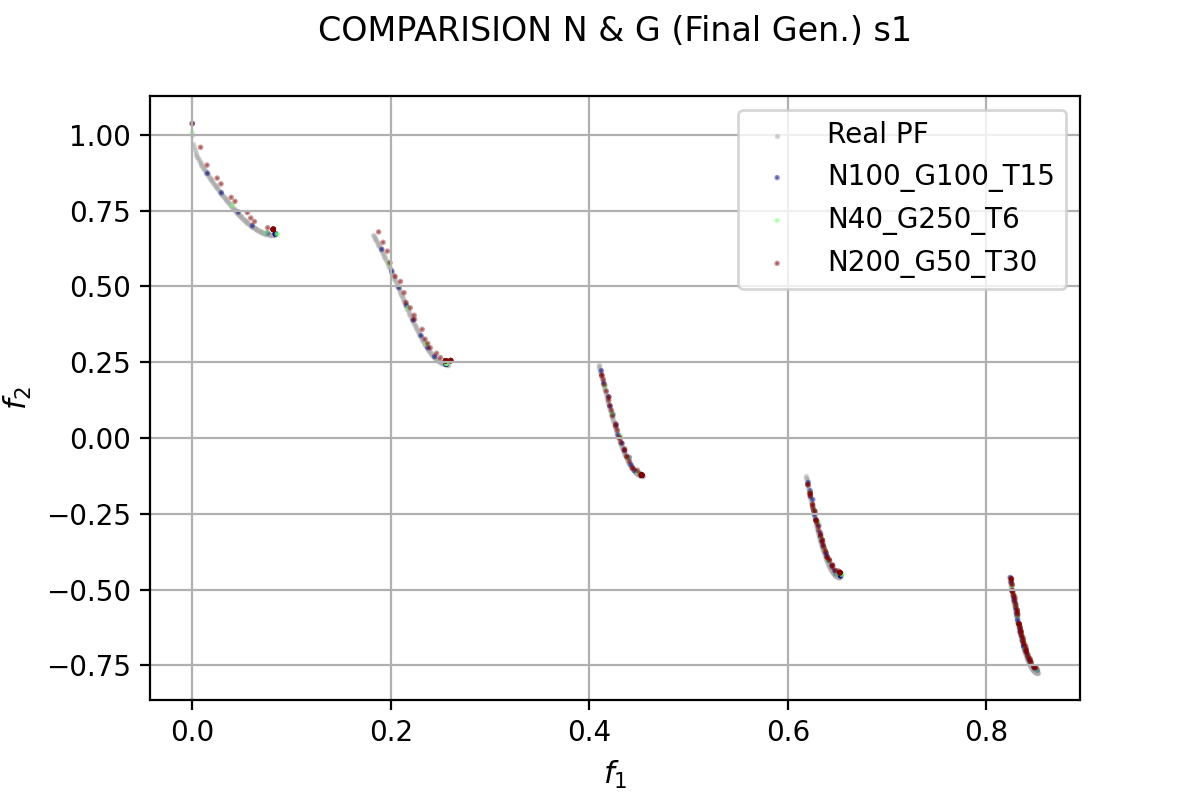
\includegraphics[scale=0.9]{figures/COMPARISIONS_EOP1/GCOMP_FGEN_s1.png}\\
\end{center}
\begin{figure}[H]
\centering
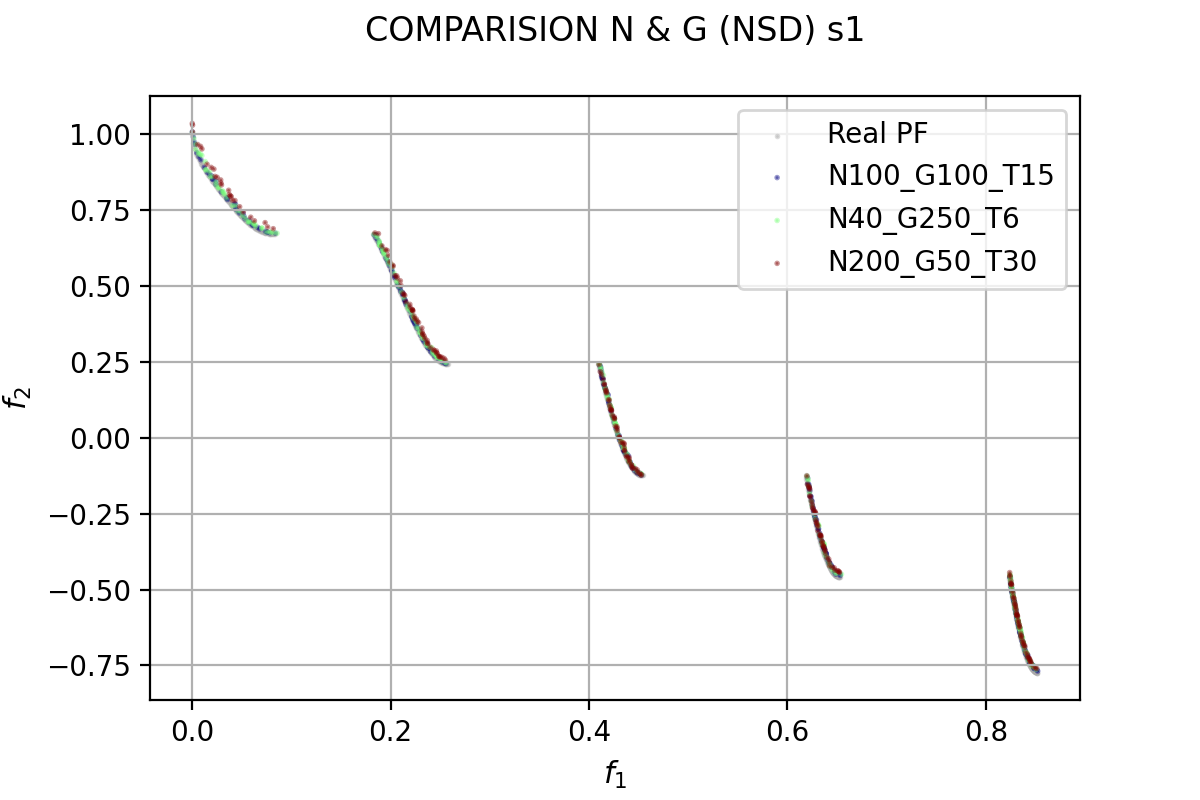
\includegraphics[scale=0.9]{figures/COMPARISIONS_EOP1/GCOMP_NDS_s1.png}\\
\caption{MOEA/D + EOP1. Comparación de casos}
\label{fig:5}
\end{figure}



\subsubsection{Análisis de métricas para 10000 ev.}

Presentado el estudio preliminar anterior vamos a tratar de profundizar para exclarecer y llevar a cabo una discusión más profunda de los casos anteriores. Para ello realizaremos un estudio de algunas métricas para los casos ya presentados. Tales métricas corresponden al hipervolumen, espaciado y cover set.\\

Comencemos viendo algunas gráficas asociadas a las métricas para los casos planteados en el apartado anterior. En la \hyperref[fig:6]{figura 6} se muestra la evolución de hipervolumen y el espaciado en durante las distintas generaciones para 10 ejecuciones del algoritmo. Podemos observar que en todos los casos  el desarrollo del hipervolumen como el del espaciado se comportan de manera bastante uniforme para todas las generaciones, lo que denota que nuestro algoritmo es robusto (aunque, lógicamente, dos ejecuciones distintas tienen comportamientos distintos, dado el carácter estocástico del algoritmo). Aunque no es posible hacer un análisis conjunto del hipervolumen (ya que el punto de referencia para su cálculo es distinto en cada caso) sí podemos destacar la rápida convergencia del algoritmo (que destacamos también en el estudio preliminar) y el aparente estancamiento final, por lo que es preferible primar el número de subproblemas frente al número de generaciones (en valores razonables)como sugiere también el comportamiento del espaciado.\\


\begin{figure}[H]
\centering
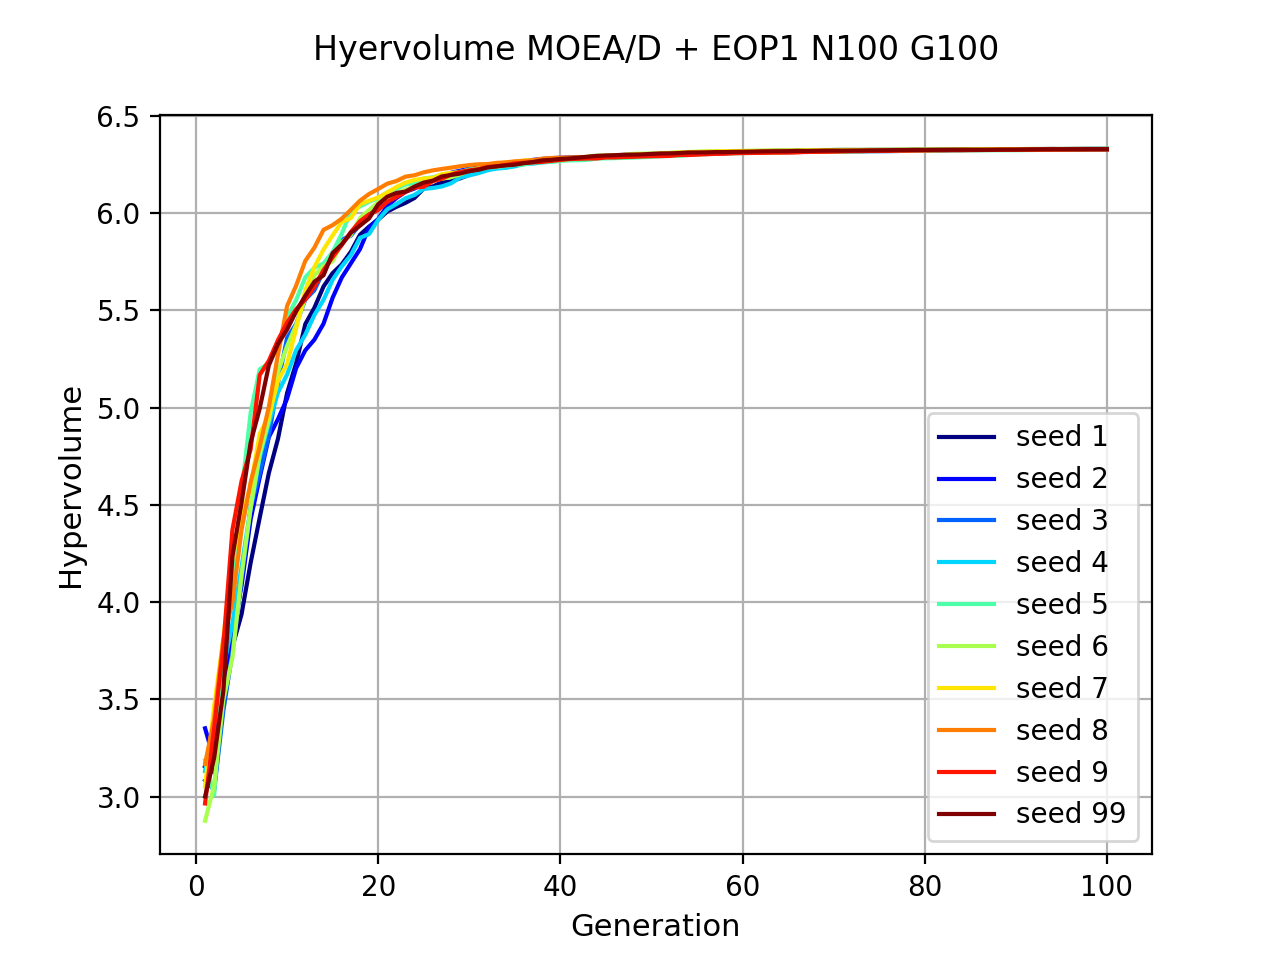
\includegraphics[scale=0.5]{figures/METRICS_EOP1/Hypervol_N100_G100.png} \quad 
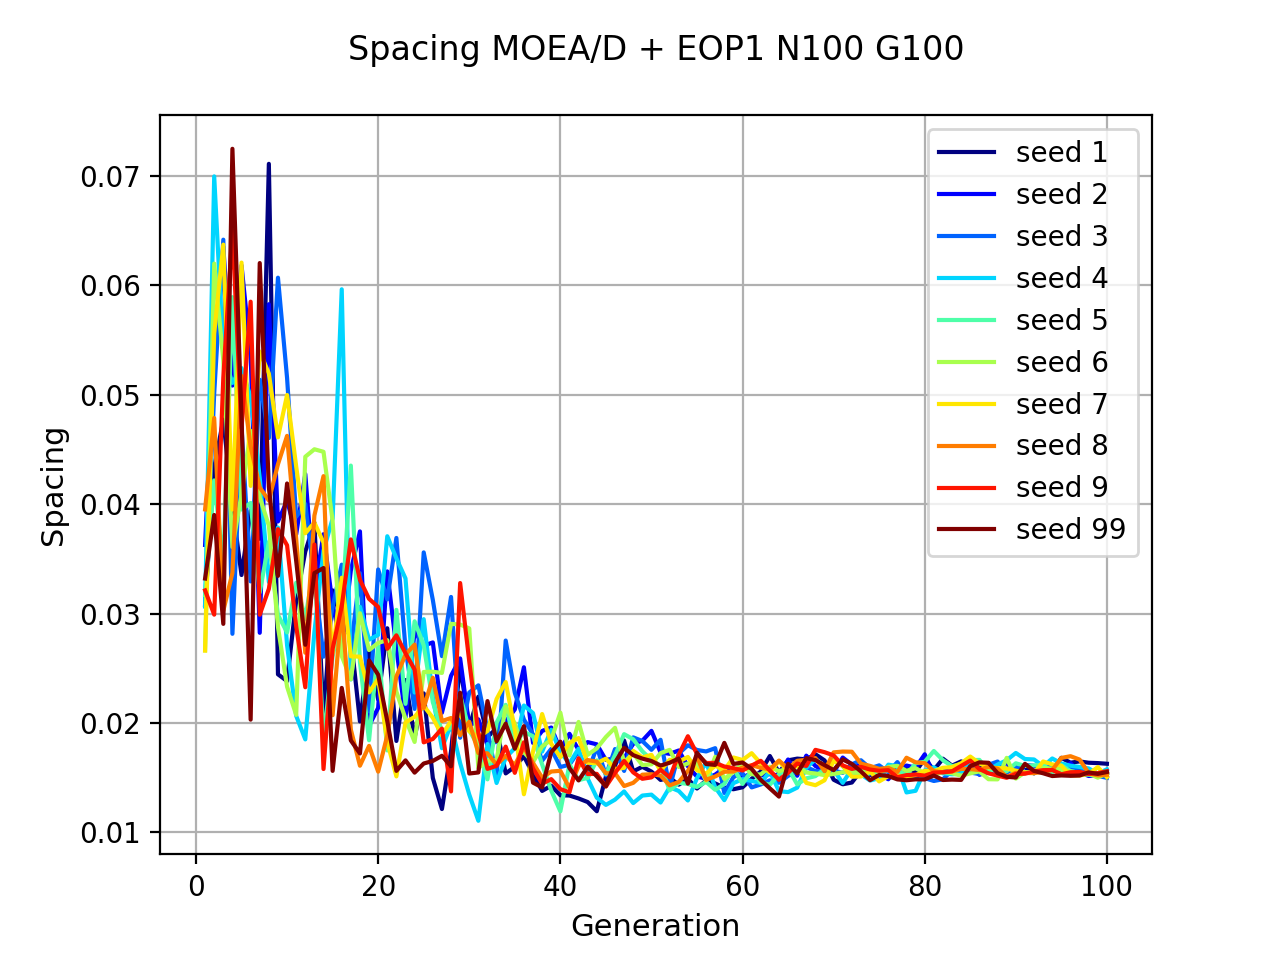
\includegraphics[scale=0.5]{figures/METRICS_EOP1/Spacing_N100_G100.png}\\
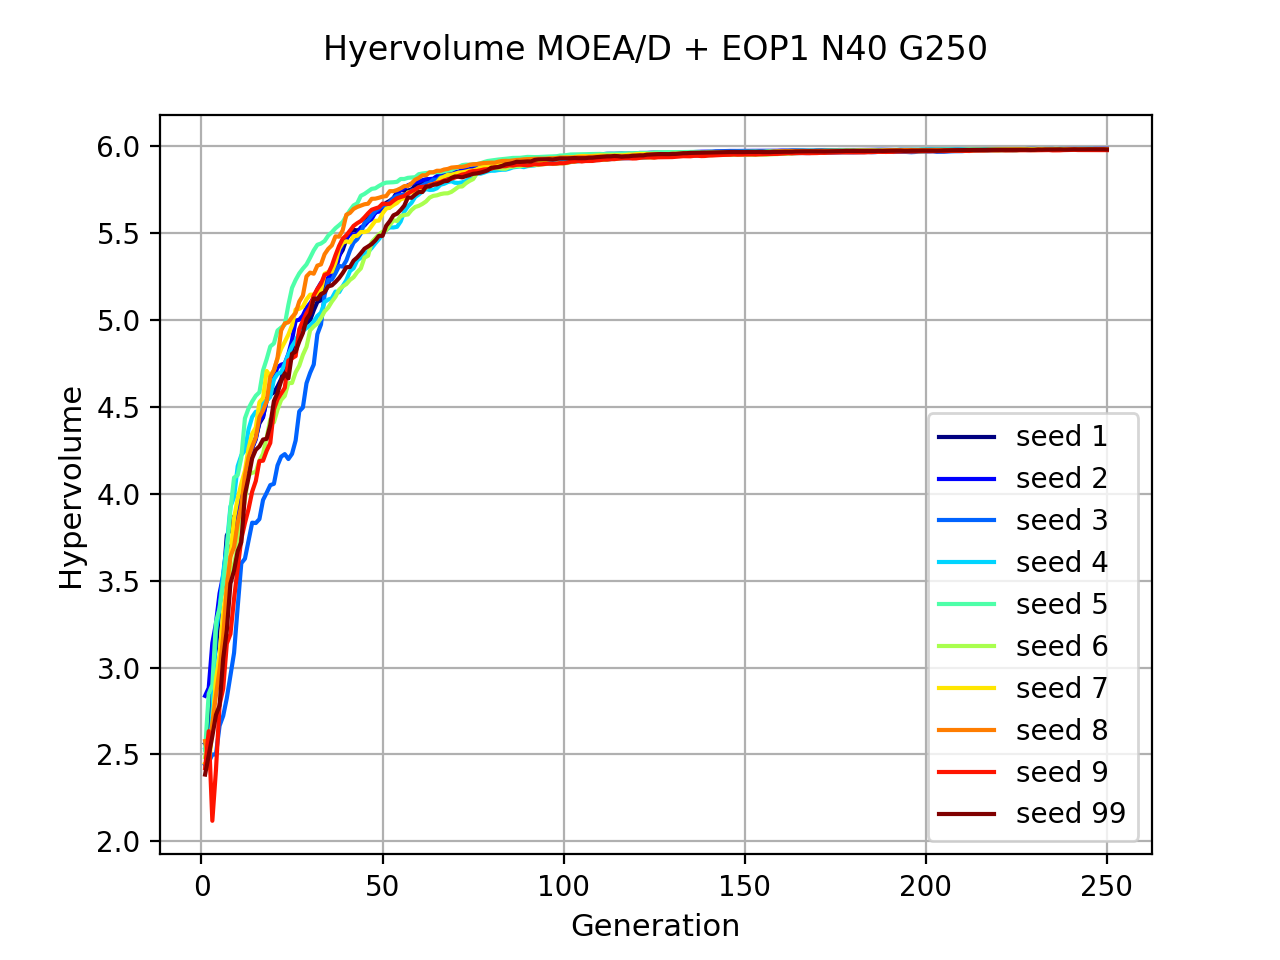
\includegraphics[scale=0.5]{figures/METRICS_EOP1/Hypervol_N40_G250.png}\quad 
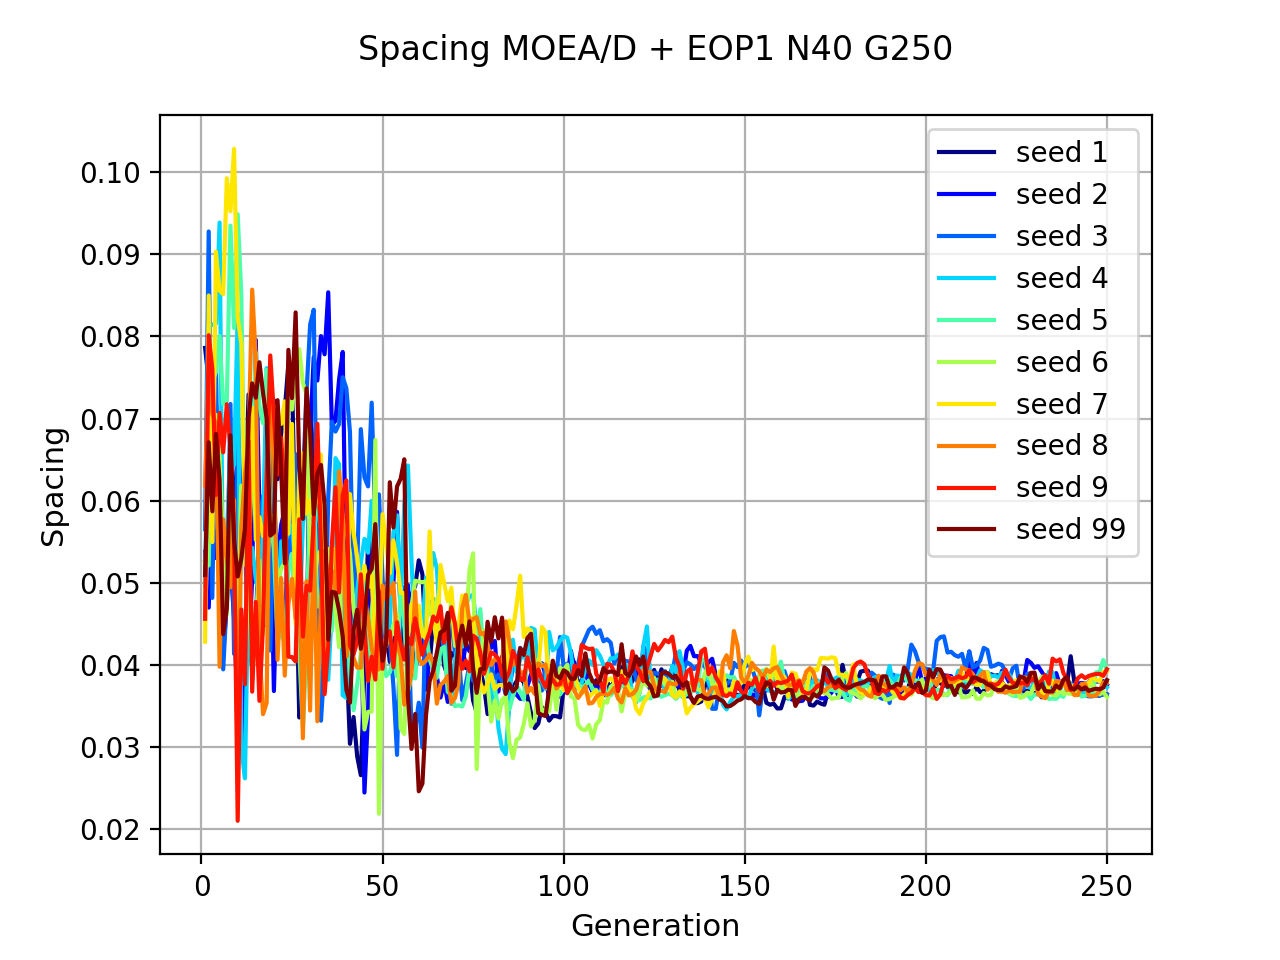
\includegraphics[scale=0.5]{figures/METRICS_EOP1/Spacing_N40_G250.png}\\
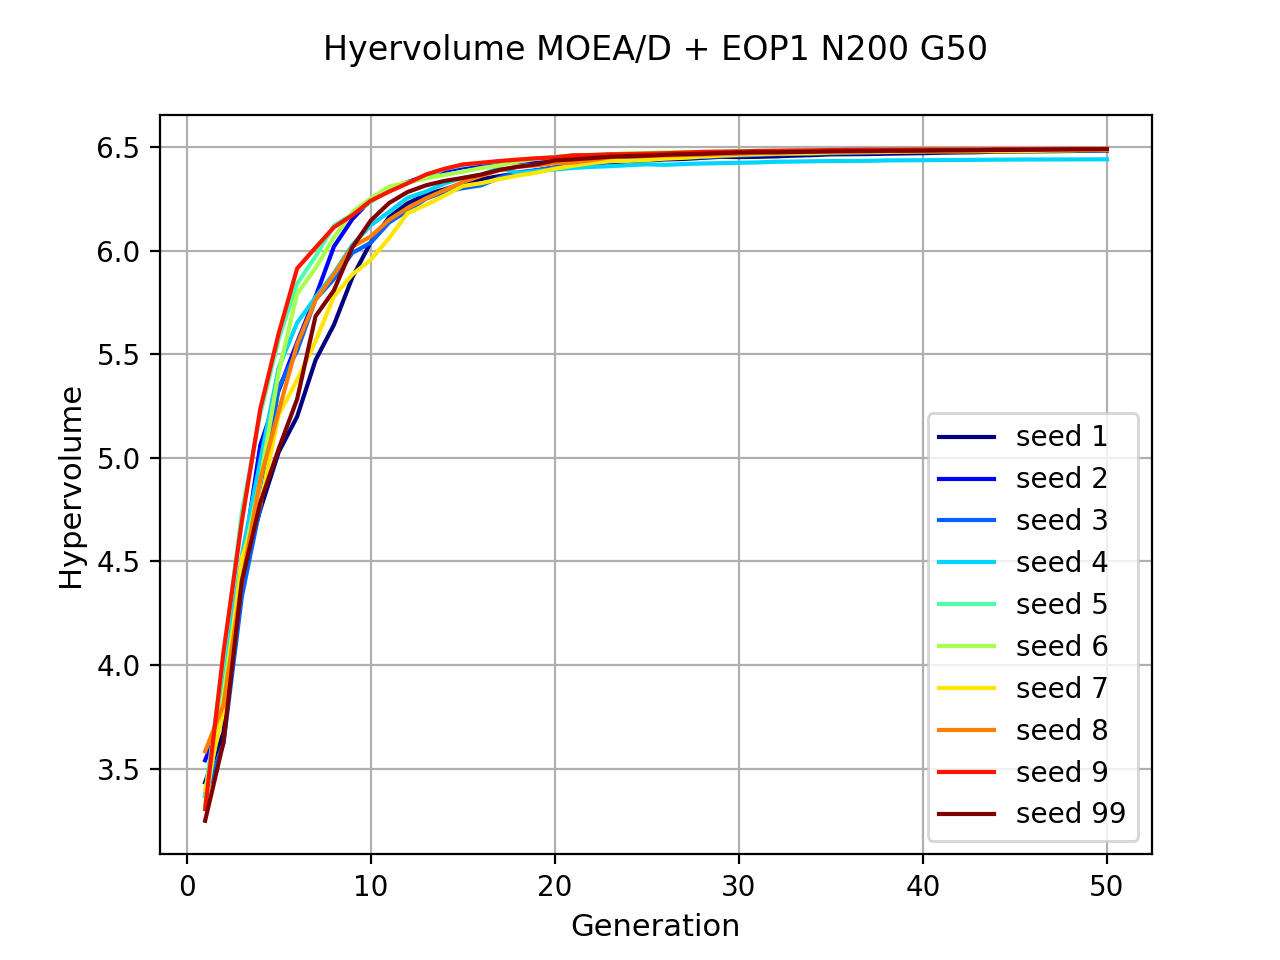
\includegraphics[scale=0.5]{figures/METRICS_EOP1/Hypervol_N200_G50.png}\quad 
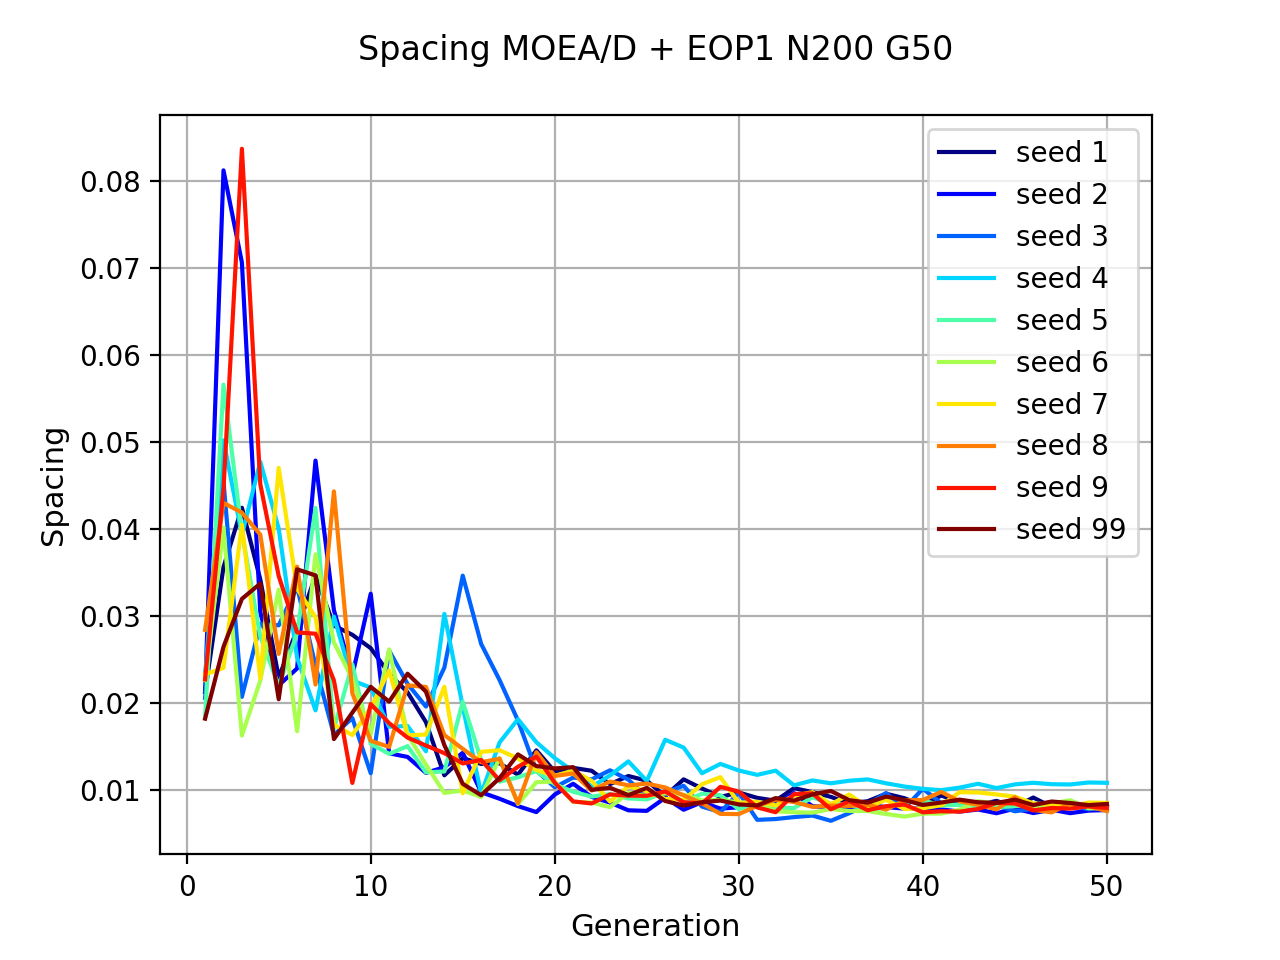
\includegraphics[scale=0.5]{figures/METRICS_EOP1/Spacing_N200_G50.png}\\
\caption{MOEA/D + EOP1. Méticas para 10000 EV}
\label{fig:6}
\end{figure}

A continuación presentaremos algunas gráficas comparativas del comportamiento del algoritmo frente a \textit{NSGAII}. En la \hyperref[fig:7]{figura 7} se muestran las graficas con dichas comparativas en las que podemos notar que en todos los casos el espaciado en el algoritmo NSGAII se compora mejor que en algoritmo propuesto mientras que el hipervolumen suele ser al revés. Como vimos en el estudio preliminar el algoritmo sí suele converger a soluciones mejores que el algoritmo \textit{NSGAII} pero también suele tender a concentrar más las soluciones. Sin embargo si comprobamos la métrica cover set, sí podemos ver que para el segundo y el tercer caso ($N100$ y $N200$) el algoritmo propuesto tiende a dominar al \textit{NSGAII}, para el primer caso en todas las ejecuciones el frente del algoritmo \textit{NSGAII} quedó dominado por el de \textit{MOEA/D + EOP1} en más del 80\% de sus puntos, mientras que el frente de  \textit{NSGAII} no es apreciable que dominase al \textit{MOEA/D + EOP1} en ni siquiera un 2\% en niguna de las ejecuciones; y además este comportamiento es patente a partir las 5 primeras iteraciones. No es así para el caso $N=40$, en el que el nuestro algorito sí supera en hipervolumen al \textit{NSGAII} pero es sensiblemente peor en cuanto al espaciado y en cuanto al cover set en ningún caso ninguno de los dos frentes es dominado más de un 40\% por el otro. aunque nuestro algoritmo tienda a quedear por debajo. Como venimos repitiendo a nuestro algoritmo le aporta más un número alto de subproblemas que de generaciones.


\begin{figure}[H]
\centering
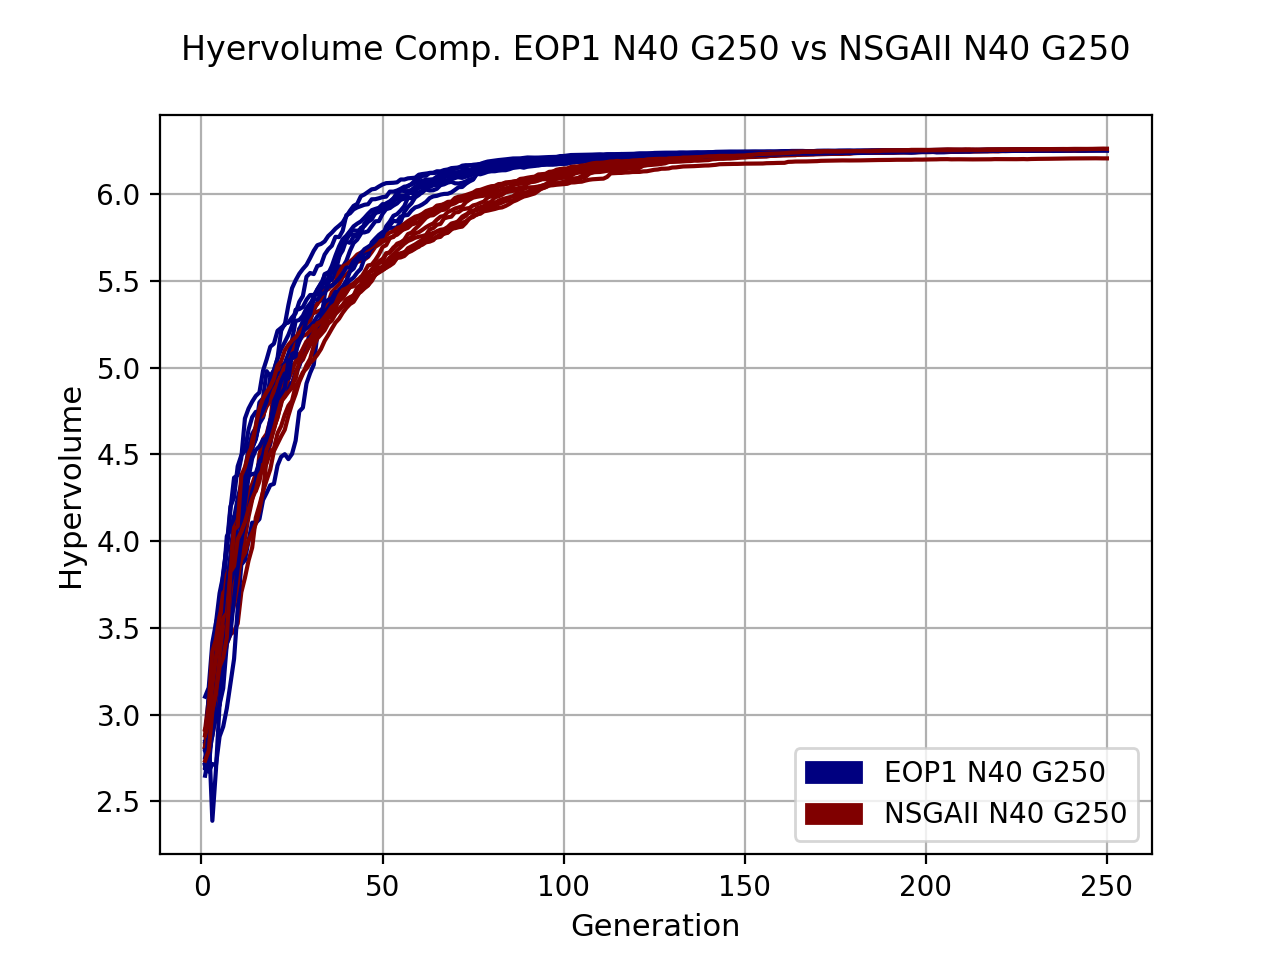
\includegraphics[scale=0.35]{../METRICS_PLOTS/Hypervol_COMP_EOP1N40G250_NSGAIIN40G250.png}
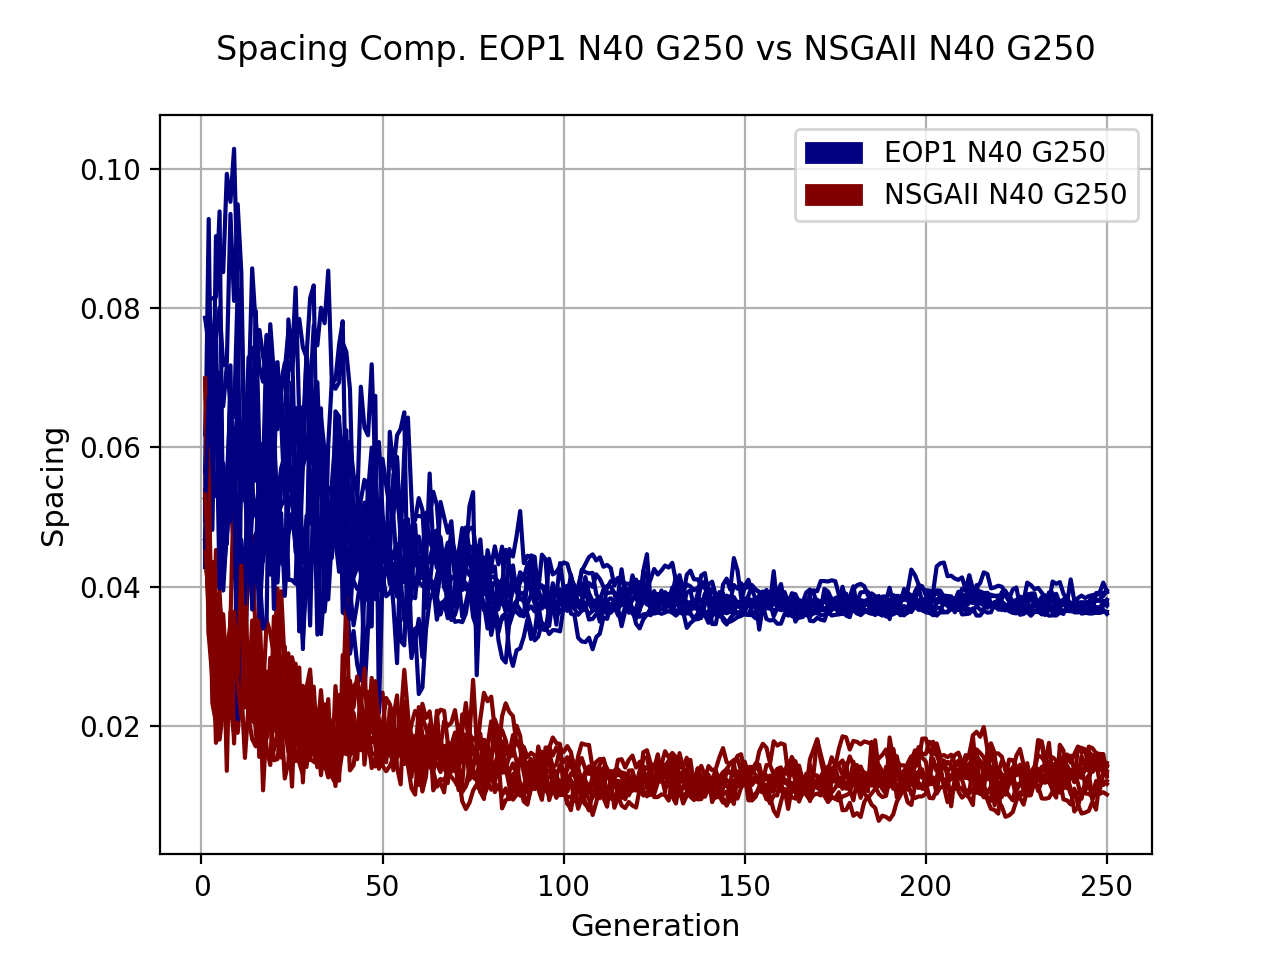
\includegraphics[scale=0.35]{../METRICS_PLOTS/Spacing_COMP_EOP1N40G250_NSGAIIN40G250.png}
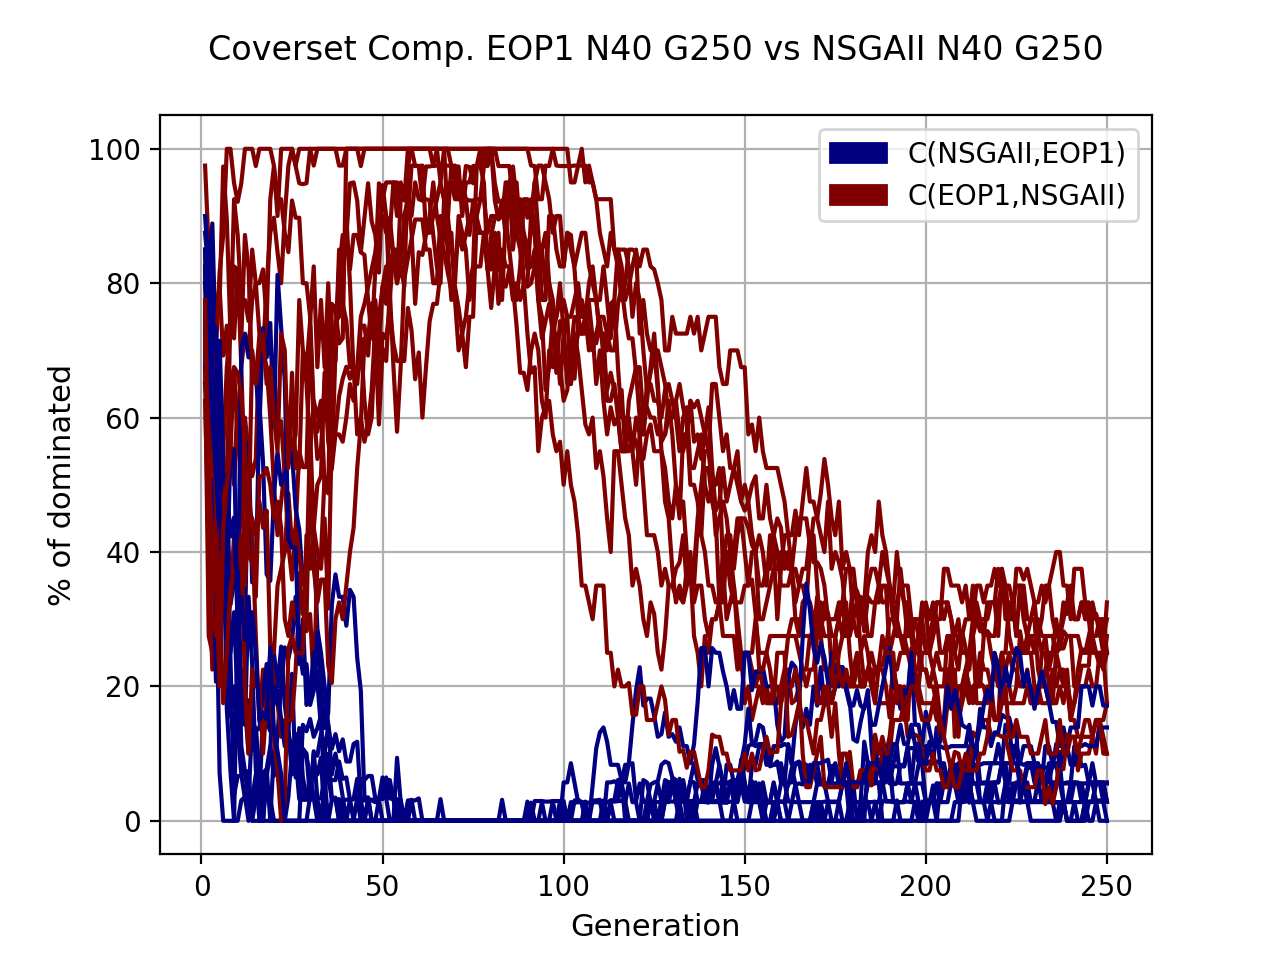
\includegraphics[scale=0.35]{../METRICS_PLOTS/CoverSet_COMP_EOP1N40G250_NSGAIIN40G250.png}\\
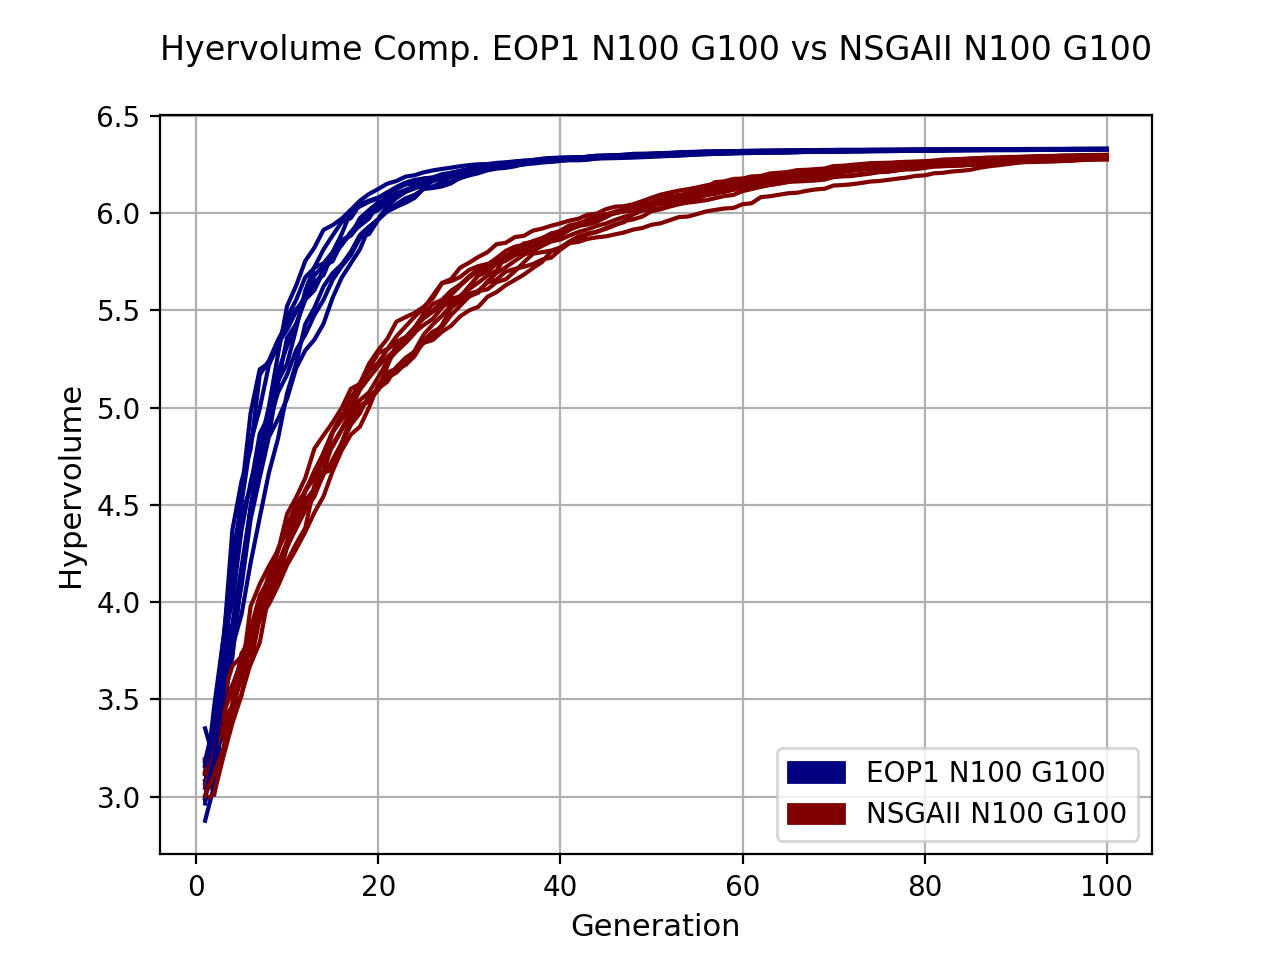
\includegraphics[scale=0.35]{../METRICS_PLOTS/Hypervol_COMP_EOP1N100G100_NSGAIIN100G100.png}
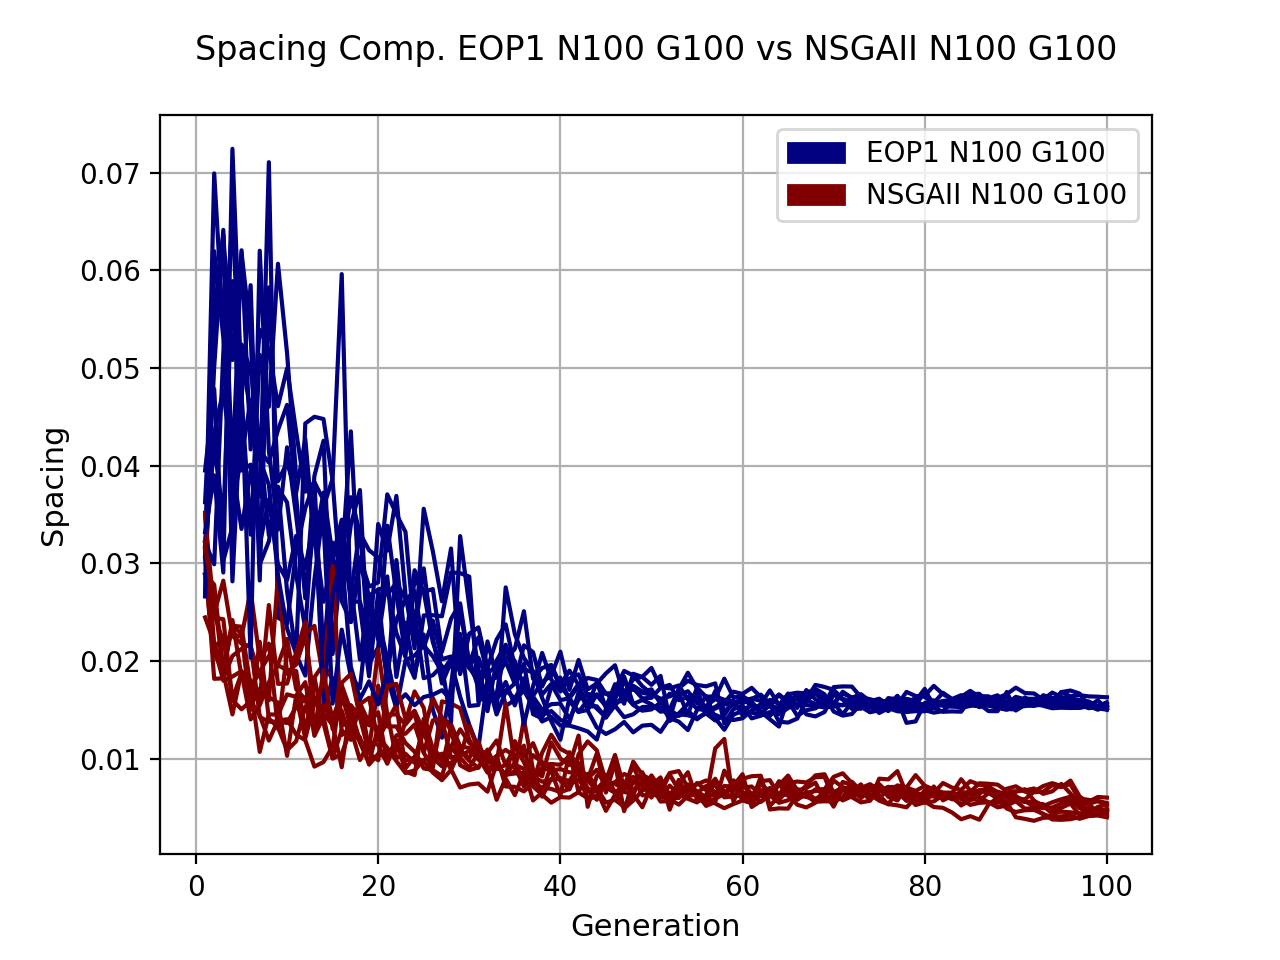
\includegraphics[scale=0.35]{../METRICS_PLOTS/Spacing_COMP_EOP1N100G100_NSGAIIN100G100.png}
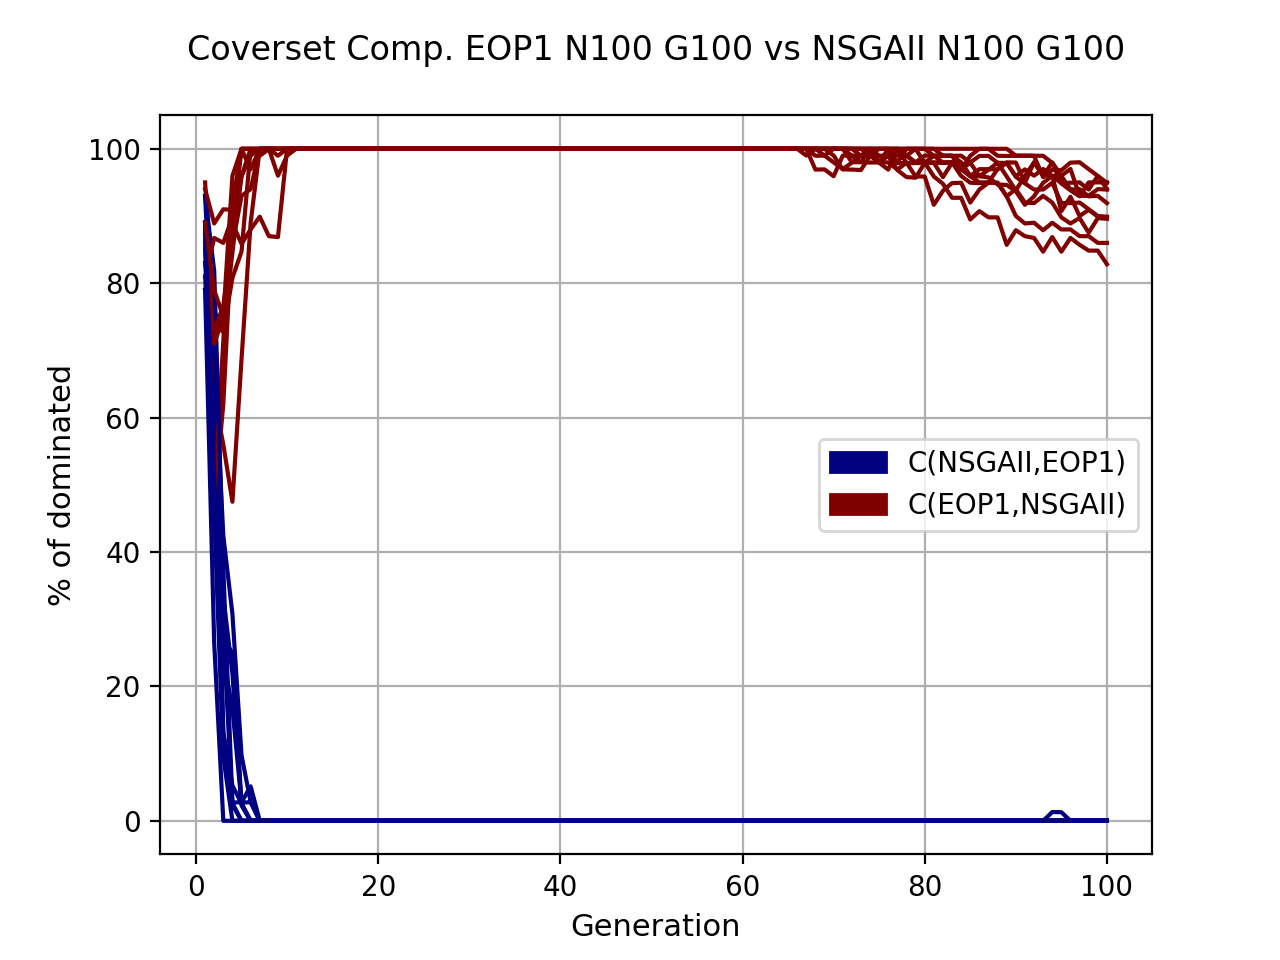
\includegraphics[scale=0.35]{../METRICS_PLOTS/CoverSet_COMP_EOP1N100G100_NSGAIIN100G100.png}\\
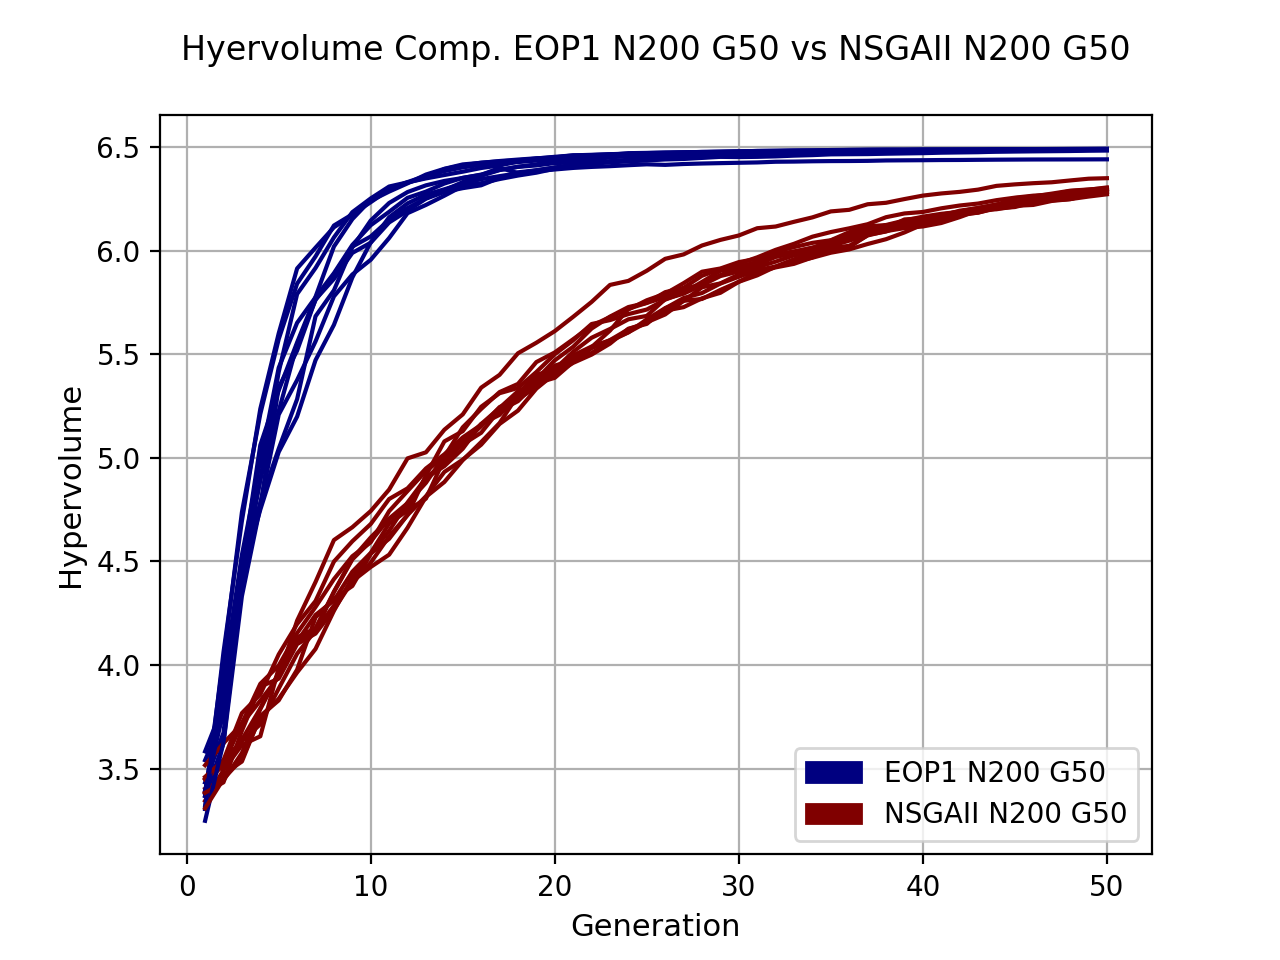
\includegraphics[scale=0.35]{../METRICS_PLOTS/Hypervol_COMP_EOP1N200G50_NSGAIIN200G50.png}
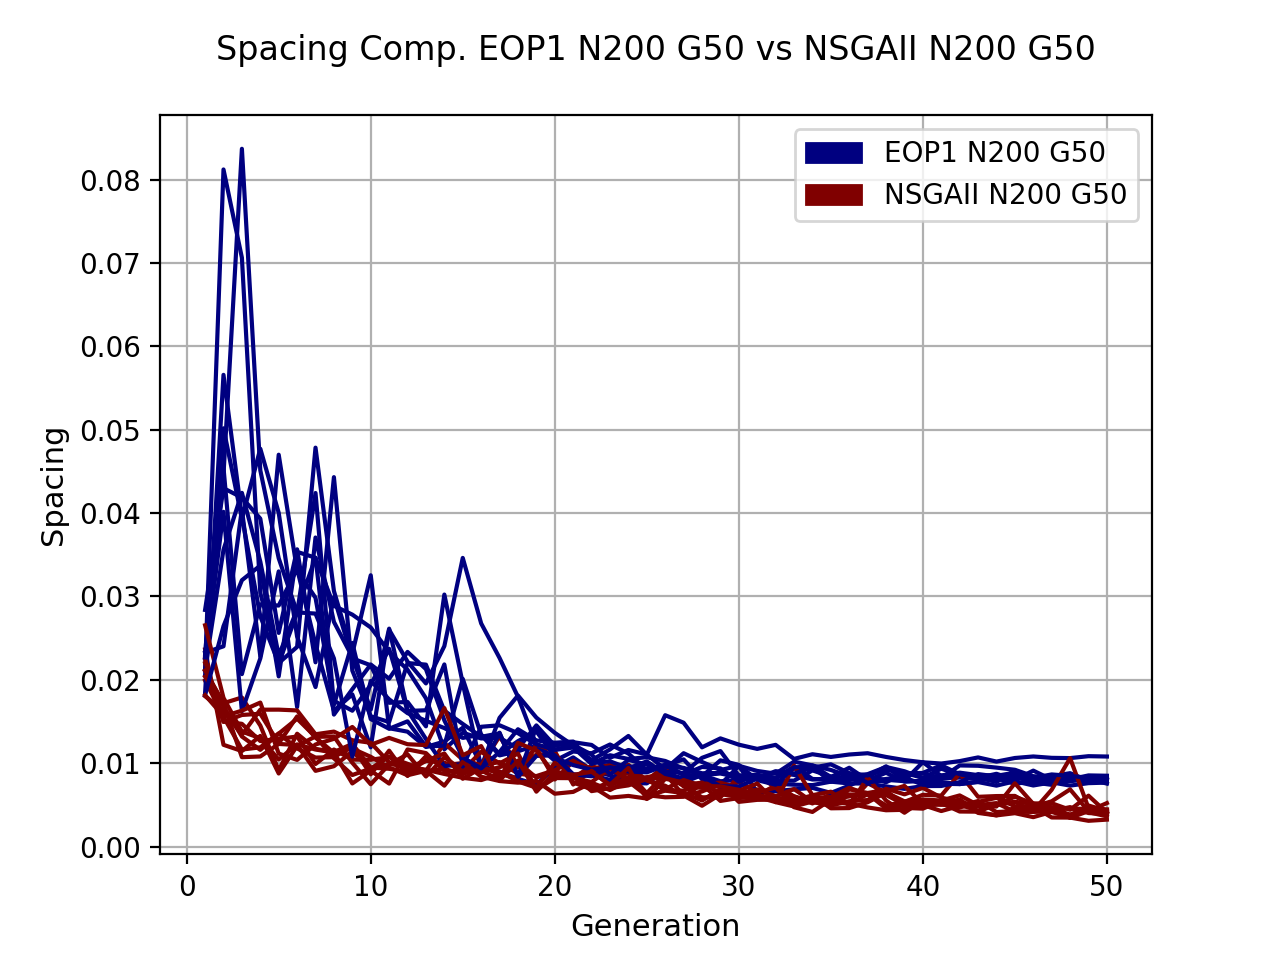
\includegraphics[scale=0.35]{../METRICS_PLOTS/Spacing_COMP_EOP1N200G50_NSGAIIN200G50.png}
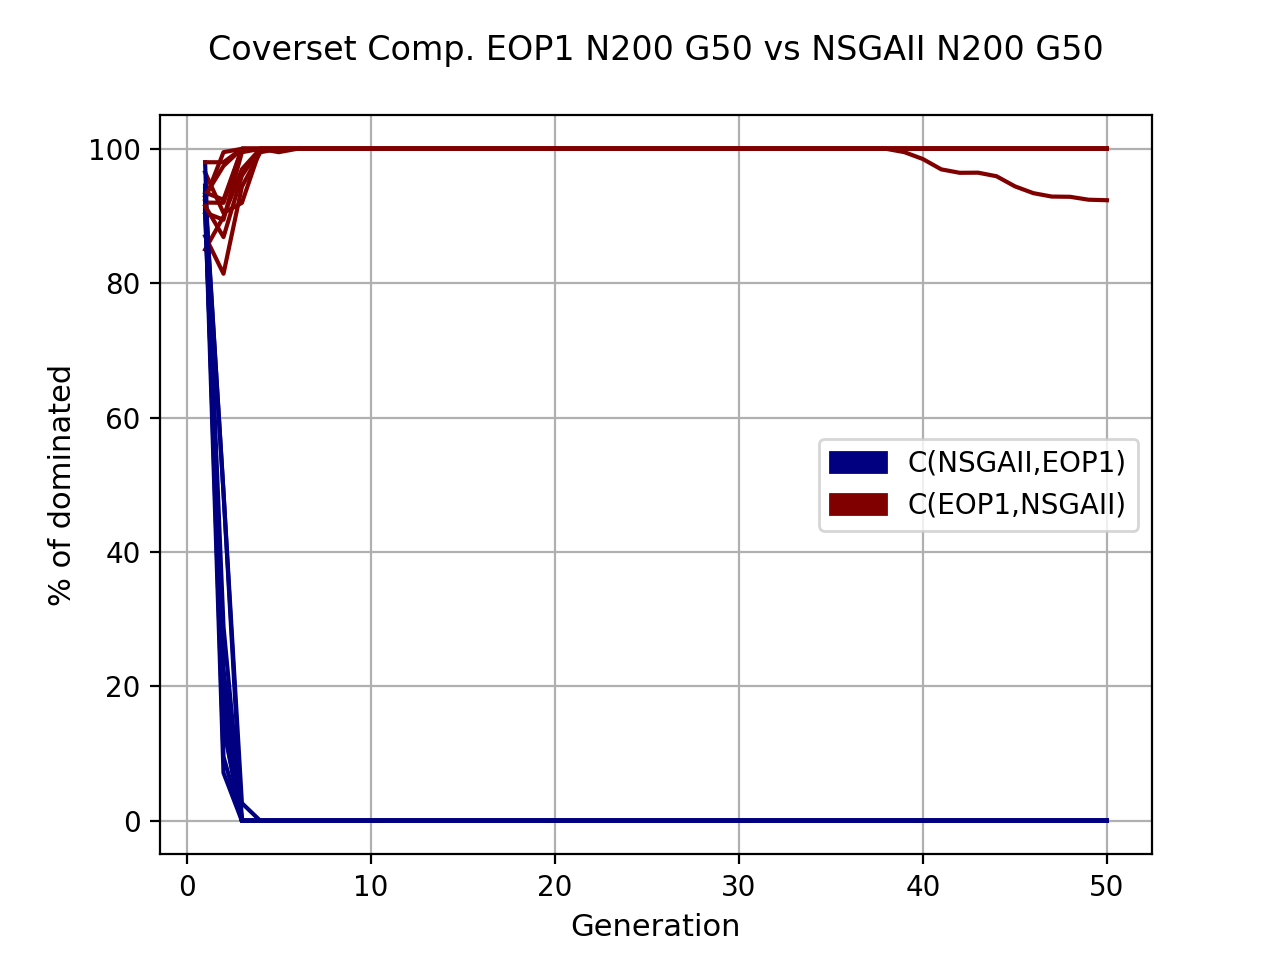
\includegraphics[scale=0.35]{../METRICS_PLOTS/CoverSet_COMP_EOP1N200G50_NSGAIIN200G50.png}\\
\caption{MOEA/D + EOP1. Comparación de métricas con NSGAII para 10000 EV.}
\label{fig:7}
\end{figure}

Aunque en este apartado no hemos realizado (explícitamente) un análisis de las soluciones (población final y NSD) en el último apartado de esta sección presentaremos una comparativa conjunta de las últimas generaciones y de los conjuntos no dominados (NSD) para todos los casos y todos los algoritmos (y operadores).

\noindent\textbf{EXPERIMENTACIÓN PARA 4000 EVALUACIONES}\\

Ya presentamos para 10000 evaluaciones el comportamiento del algoritmo es adecuado, esto es, a través de las generaciones los individuos se aproximan al frente. No vamos a volver a presentarlo para el caso de 4000 evaluaciones, pues sigue lógicamente el mismo esquema (en los apéndices se presentan las gráficas que atestiguan lo expuesto). Por tanto pasaremos directamente a evaluar las métricas y a razonar directamente sobre los resultados obtenidos en dicho análisis.  \\

En la \hyperref[fig:8]{figura 8} se presentan las gráficas del desarrollo del hypervolumen y el espaciado para cada uno de los casos coniderados en las 4000 evaluaciones en contreto $(N=40, G=100)$, $(N=80, G=50)$, $(N=100, G=40)$. Como podemos apreciar el comportamiento es similar a los presentados para las 10000 evaluaciones, denotándose que la convergencia (hipervolumen) se desarrolla de forma análoga a como lo hacía para los casos previos (viendo la forma de la curva, dado que los valores no son comparables debido a la desigualdad del punto de referencia en cada caso), pero truncada a las iteraciones correspondientes (aproximadamente). De igual forma el espaciado disminuye notablemente con el aumento del número de subproblemas, lo que sin duda se adecua a los resultados presentados previamente.\\

Si realizamos una comparativa (al igual que en el caso de 10000 ev) con el algoritmo \textit{NSGAII} obtenemos conclusiones análogas a las ya presentadas previamente, descando que en cuanto a convergencia en todos los casos nuestro algoritmo supera al algoritmo \textit{NSGAII}, en espaciado ocurre al contrario y en cuanto al cover set, para el caso $N=40$ el frente más del 50\%   del frente (final) de \textit{NSGAII} es dominado por el de nuestro algoritmo, mientras que apenas un 5\% del frente de nuestro algoritmo es dominado por el competidor. En los otros dos casos el cover set es mucho más claro de forma que aparentemente (para ambos casos) el 100\% del frente es dominado (en todas las ejecuciones) por el frente final (última generación) de nuestro algoritmo y mientras que para ningún punto (o desde luego menor al 1\% o 2\%) se da el comportamiento contrario.\\

De todo ello destacamos la bondad de nuestro algoritmo en cuanto a la convergencia, no tanto para el espaciado (sobre todo si consideramos la última generación, si consideramos el frente NSD veremos que el espaciado mejora notablemente, presentado en la comparativa final de la \hyperref[table:1]{tabla 1}) y en cuanto al cover set, con el número adecuado de subproblemas (mejor que de generaciones) nuestro algoritmo domina practicamente en su totalidad a \textit{NSGAII}. \\

\begin{center}
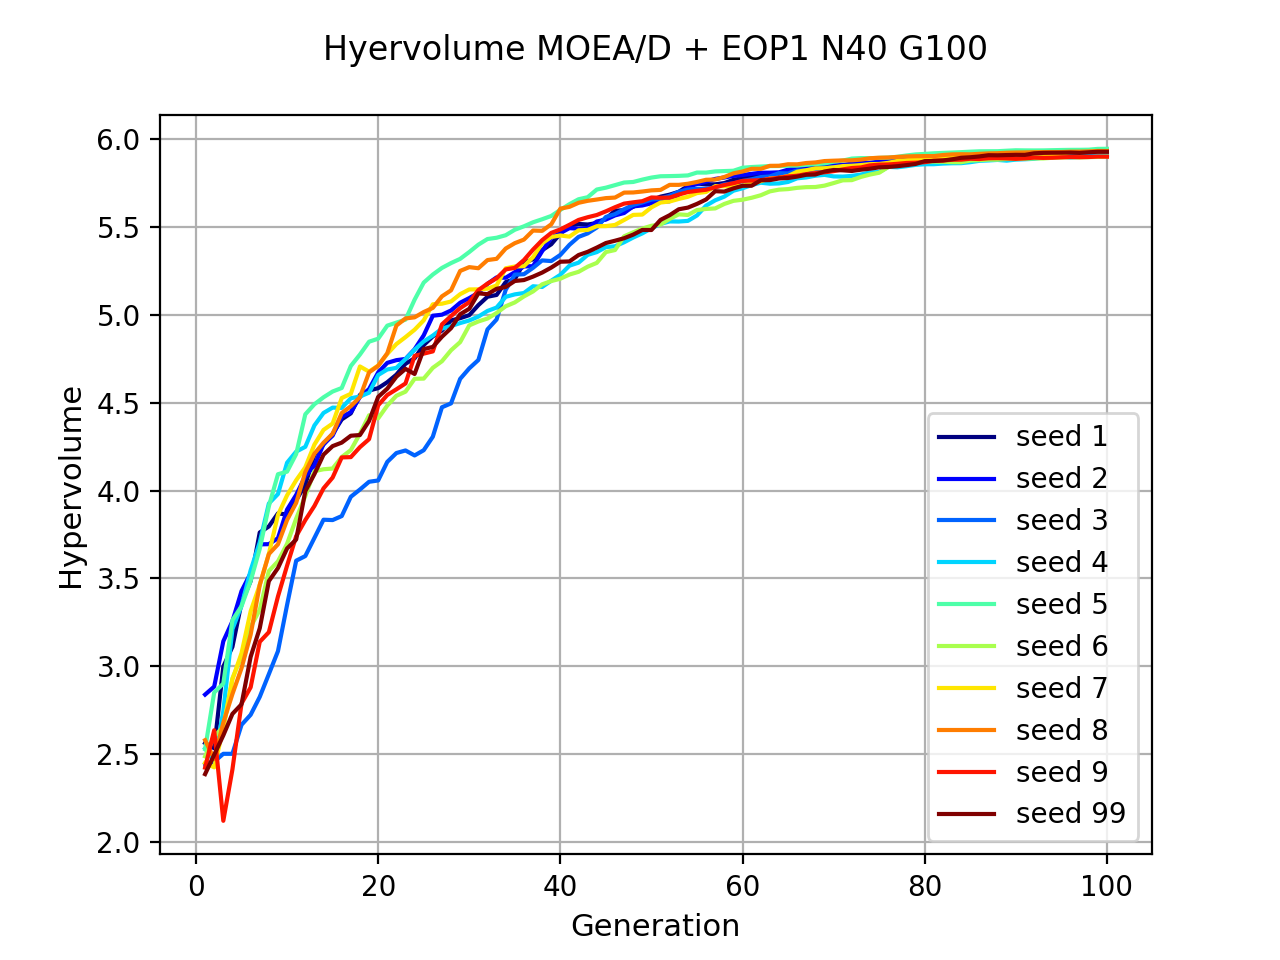
\includegraphics[scale=0.43]{figures/METRICS_EOP1/Hypervol_N40_G100.png} \quad 
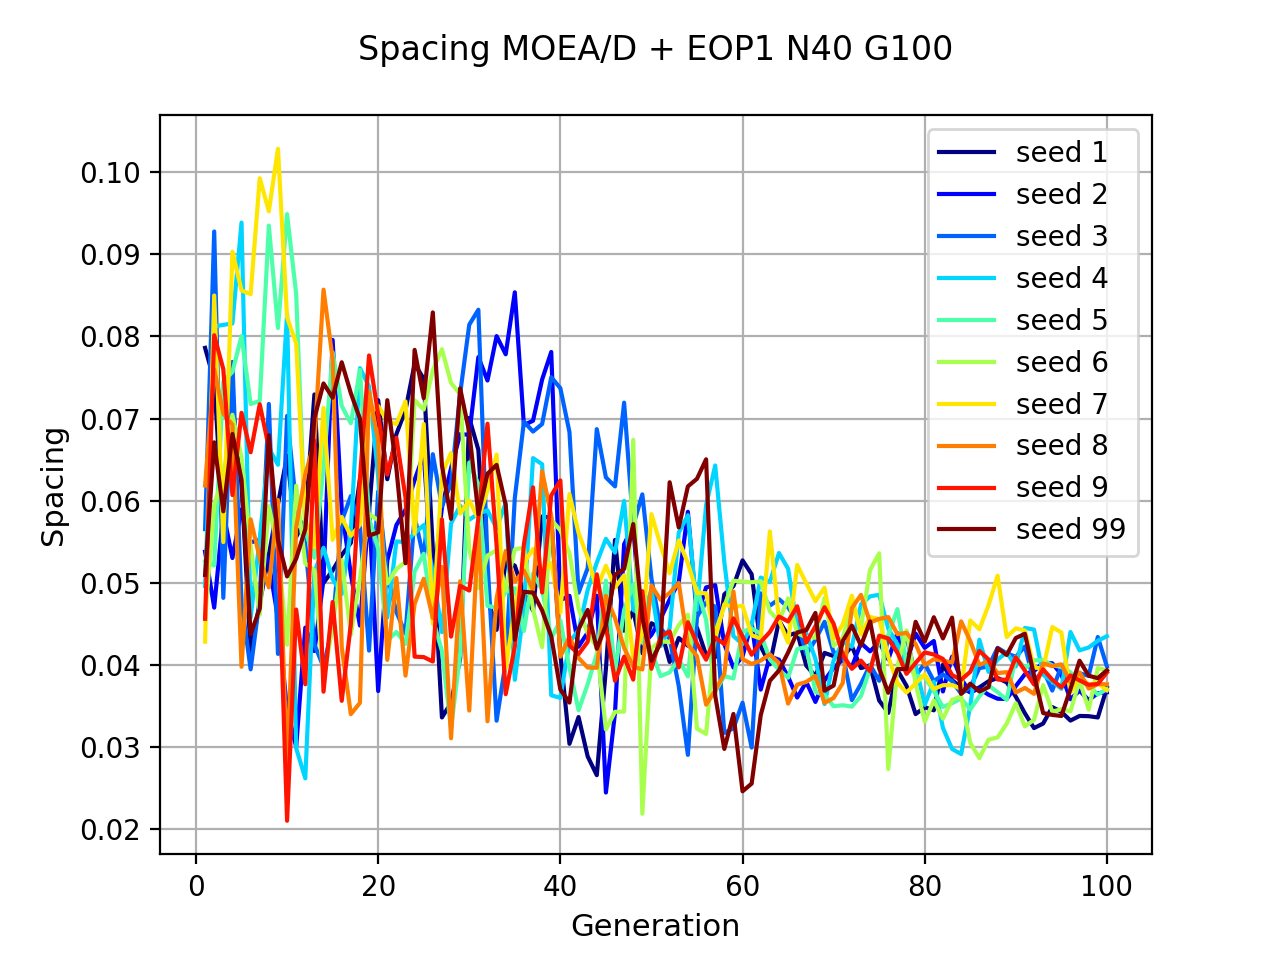
\includegraphics[scale=0.43]{figures/METRICS_EOP1/Spacing_N40_G100.png}\\
\end{center}

\begin{figure}[H]
\centering
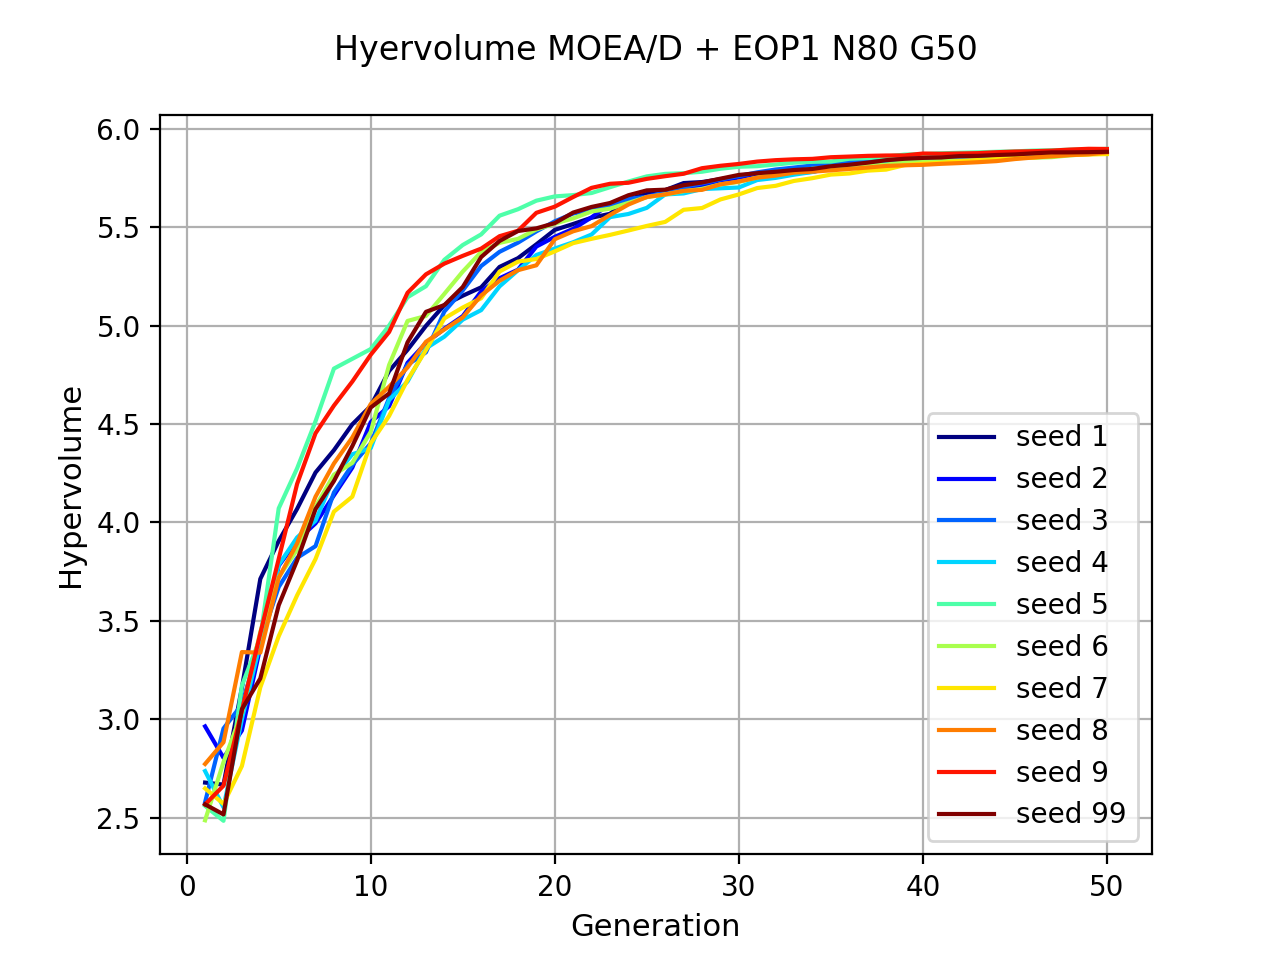
\includegraphics[scale=0.43]{figures/METRICS_EOP1/Hypervol_N80_G50.png}\quad 
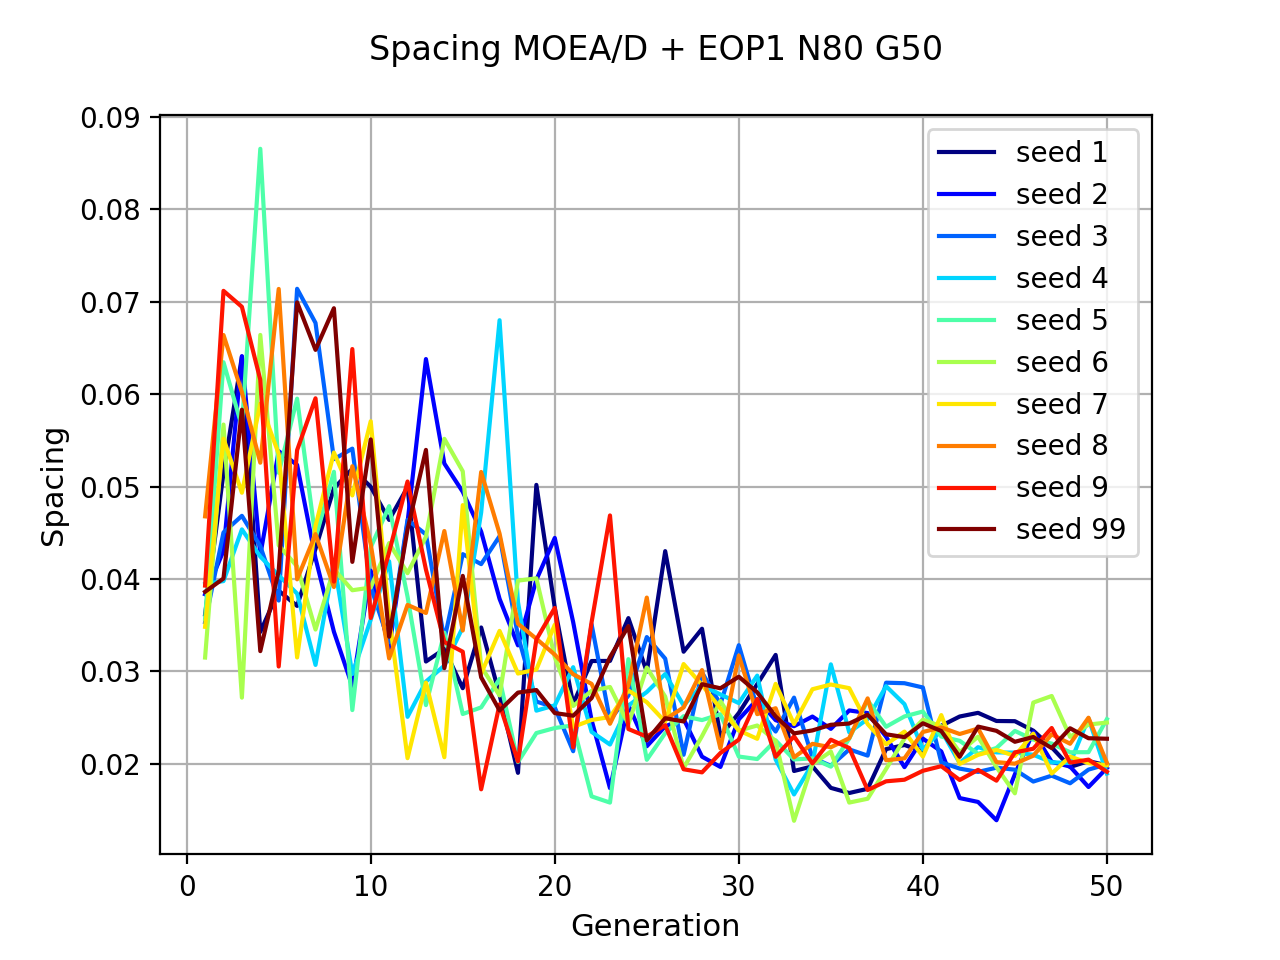
\includegraphics[scale=0.43]{figures/METRICS_EOP1/Spacing_N80_G50.png}\\
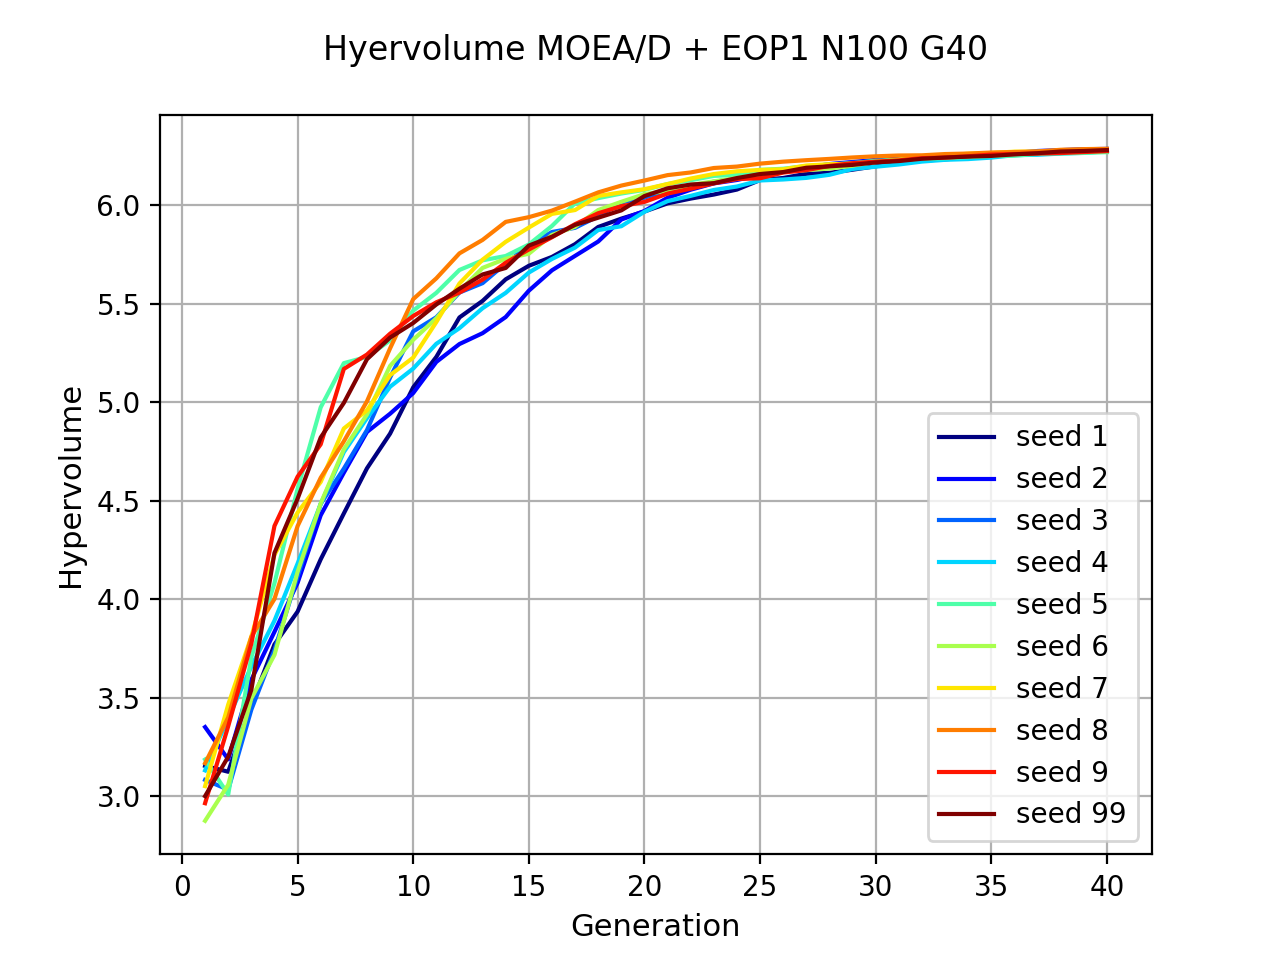
\includegraphics[scale=0.43]{figures/METRICS_EOP1/Hypervol_N100_G40.png}\quad 
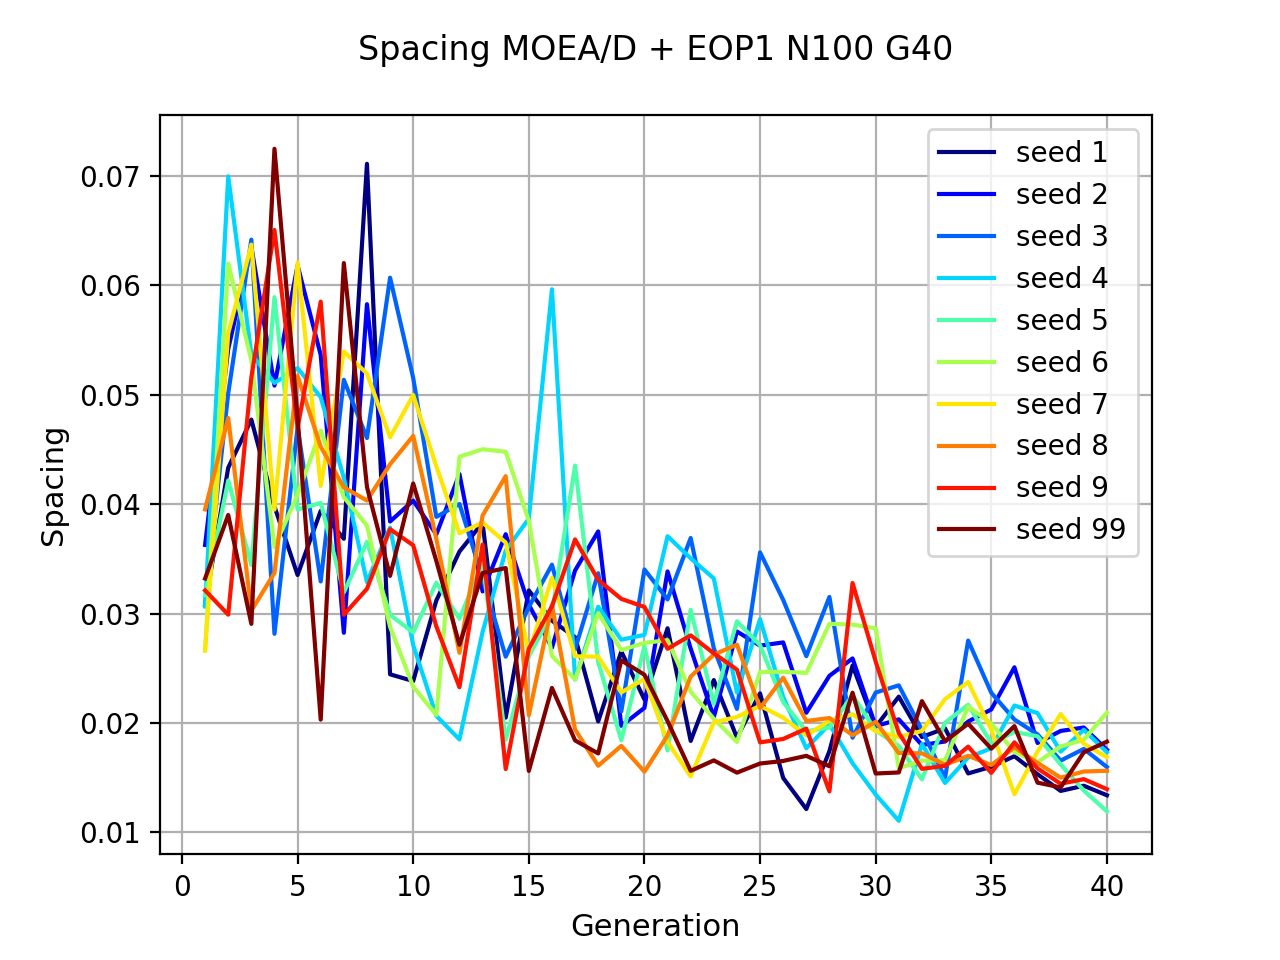
\includegraphics[scale=0.43]{figures/METRICS_EOP1/Spacing_N100_G40.png}\\
\caption{MOEA/D + EOP1. Métricas para 4000EV}
\label{fig:8}
\end{figure}

\hfill\break

\begin{center}
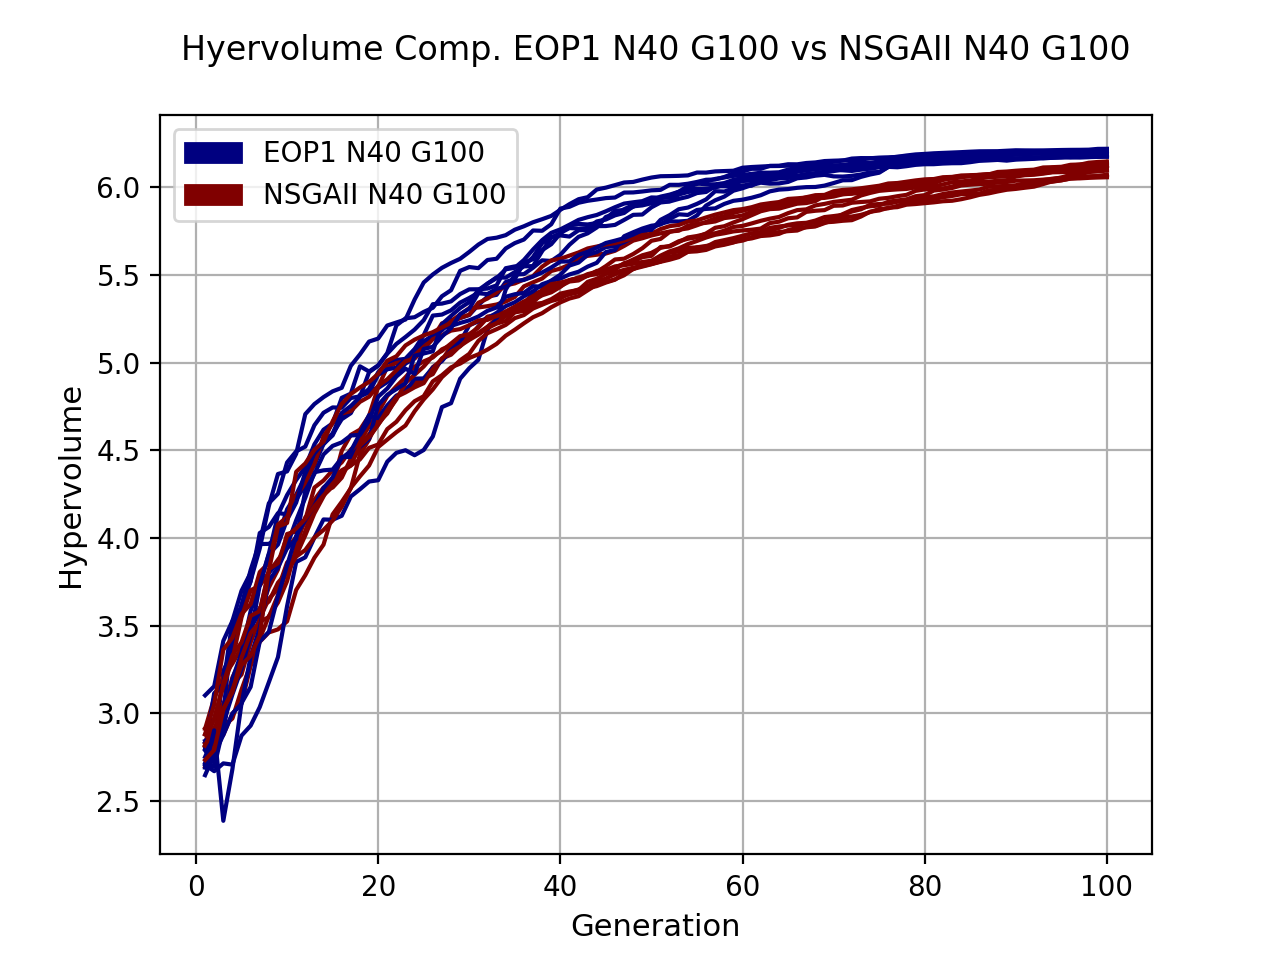
\includegraphics[scale=0.35]{../METRICS_PLOTS/Hypervol_COMP_EOP1N40G100_NSGAIIN40G100.png}
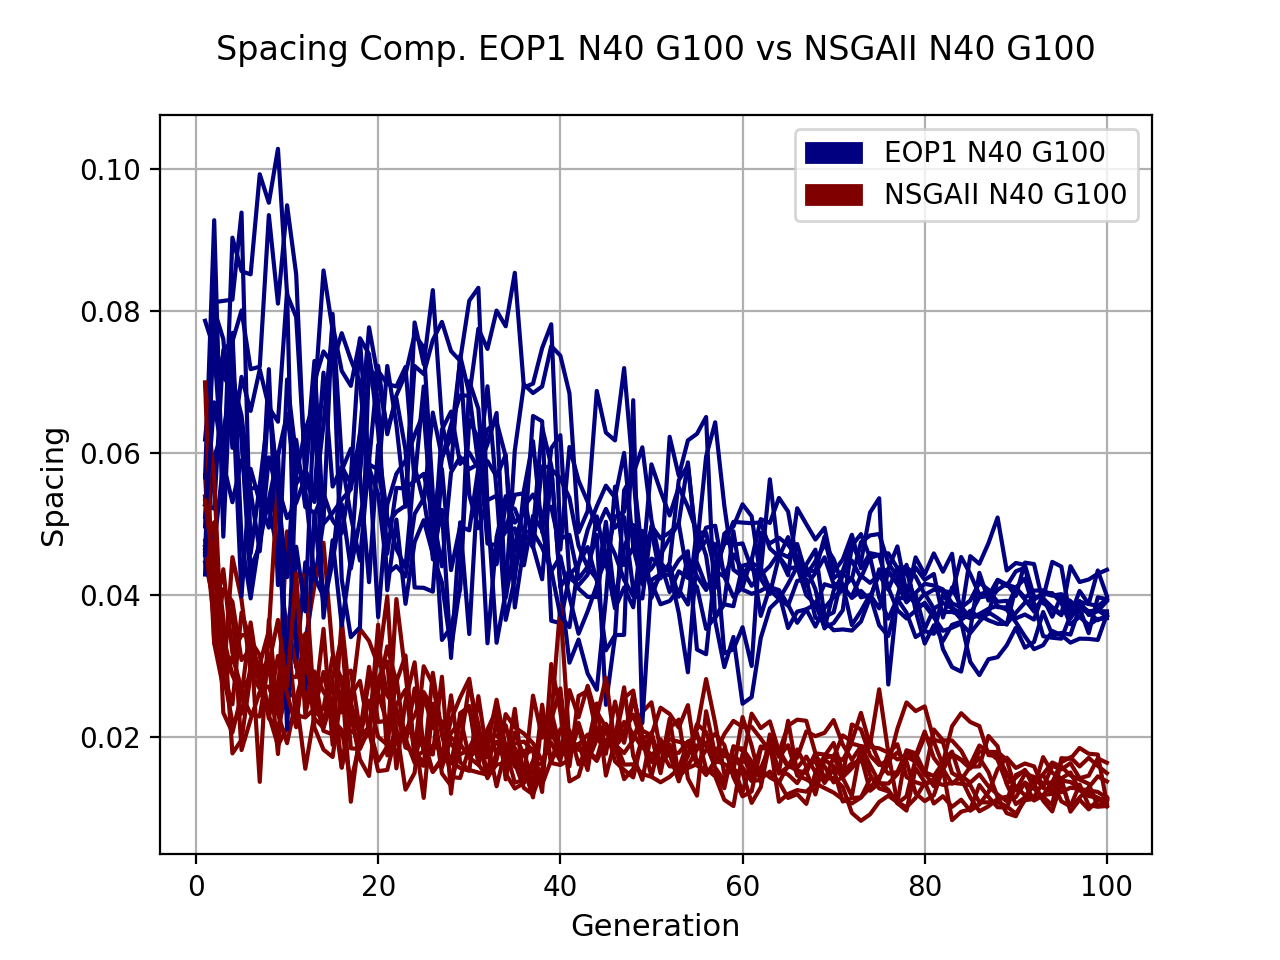
\includegraphics[scale=0.35]{../METRICS_PLOTS/Spacing_COMP_EOP1N40G100_NSGAIIN40G100.png}
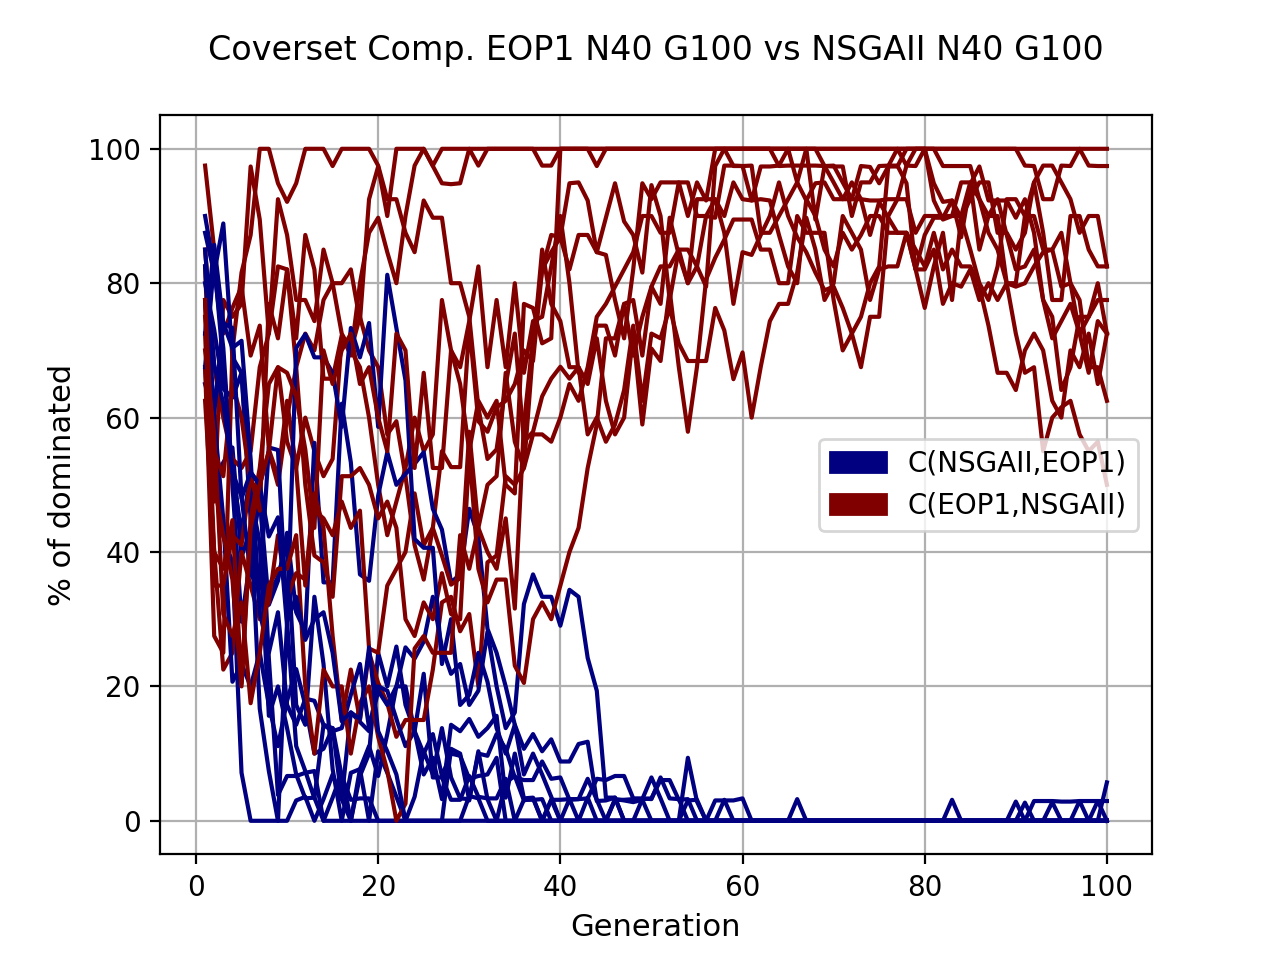
\includegraphics[scale=0.35]{../METRICS_PLOTS/CoverSet_COMP_EOP1N40G100_NSGAIIN40G100.png}\\
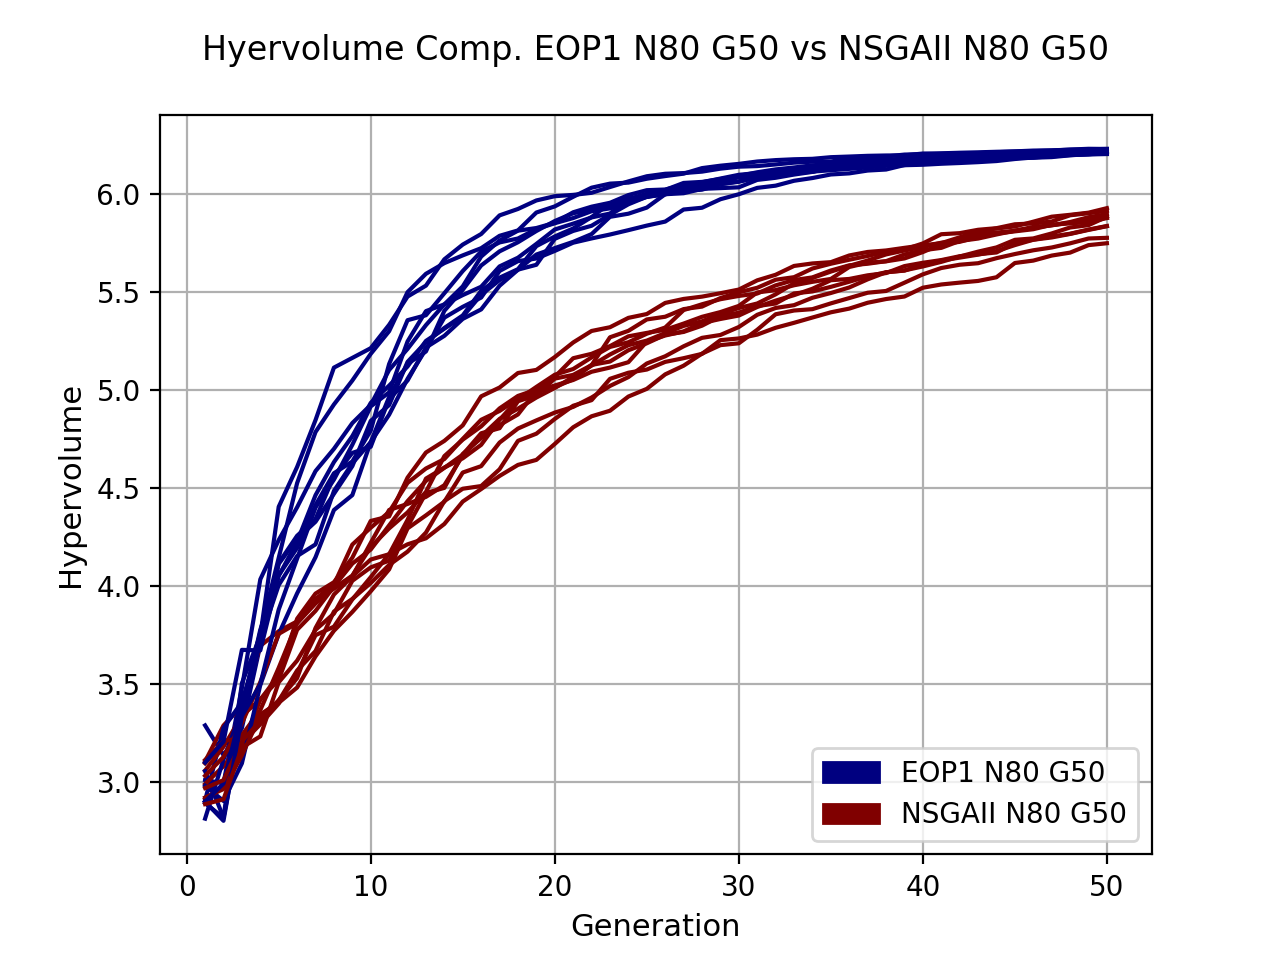
\includegraphics[scale=0.35]{../METRICS_PLOTS/Hypervol_COMP_EOP1N80G50_NSGAIIN80G50.png}
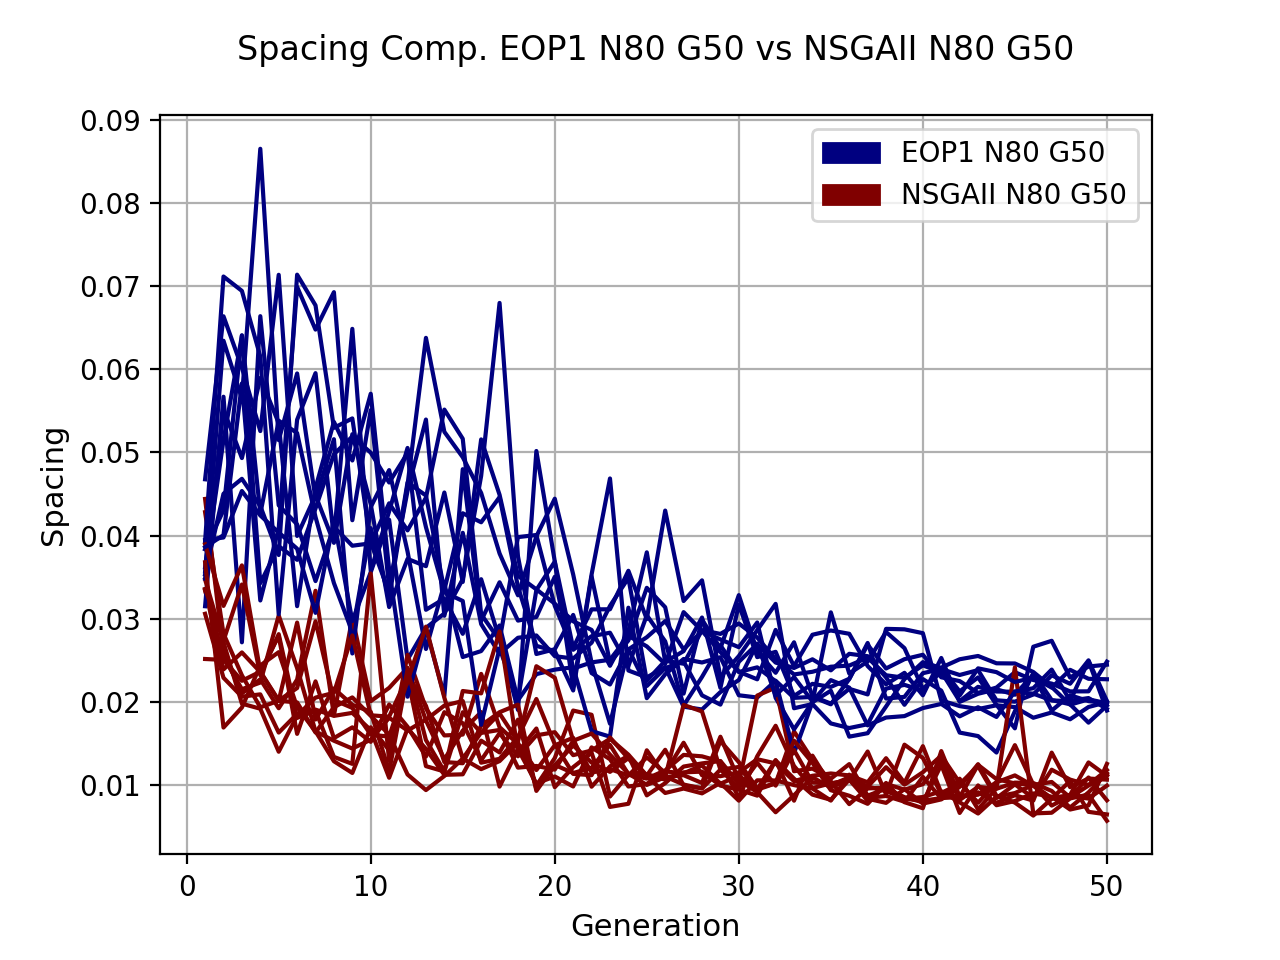
\includegraphics[scale=0.35]{../METRICS_PLOTS/Spacing_COMP_EOP1N80G50_NSGAIIN80G50.png}
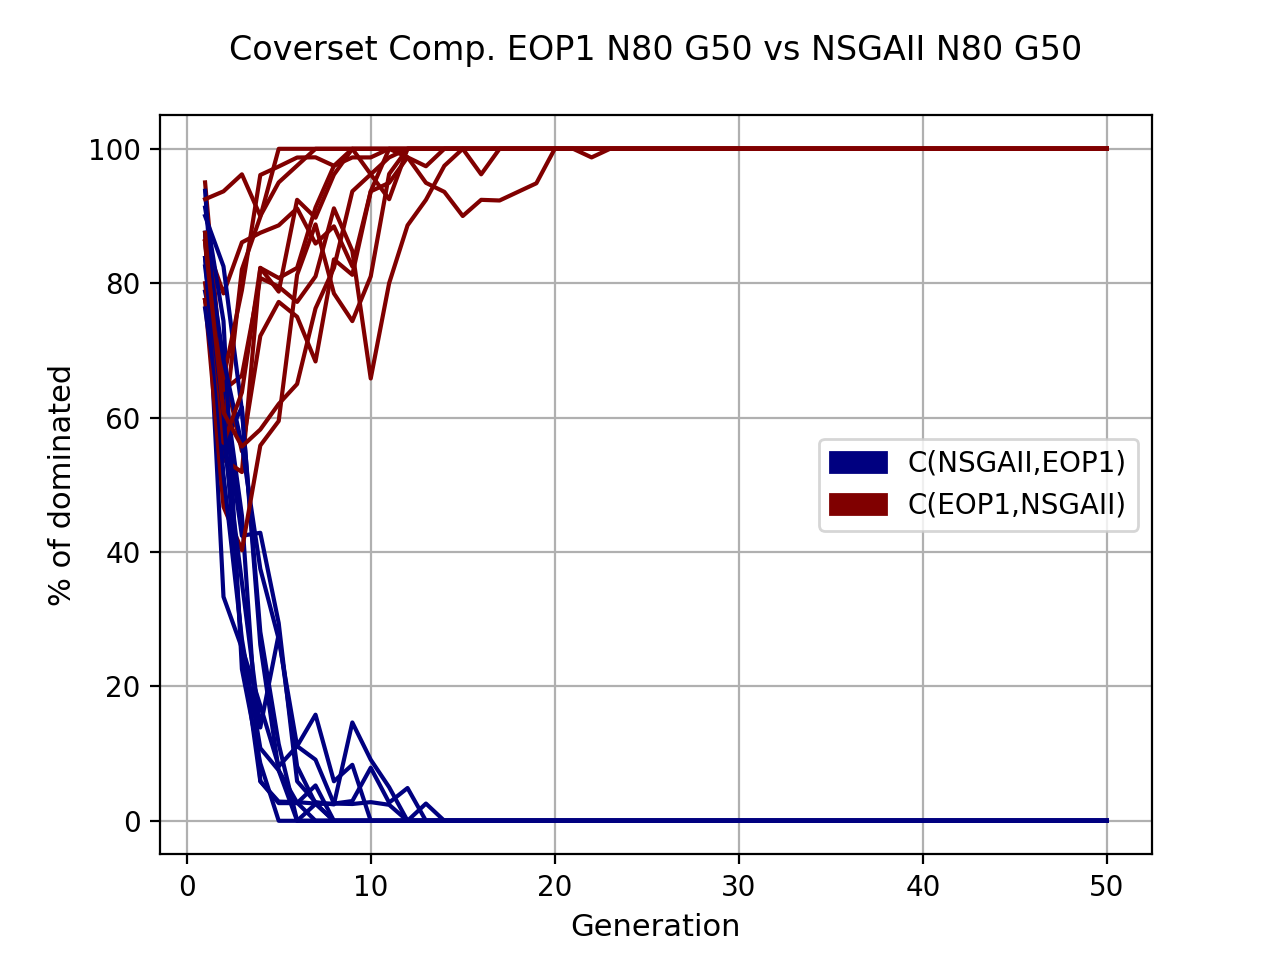
\includegraphics[scale=0.35]{../METRICS_PLOTS/CoverSet_COMP_EOP1N80G50_NSGAIIN80G50.png}\\
\end{center}

\begin{figure}[H]
\centering
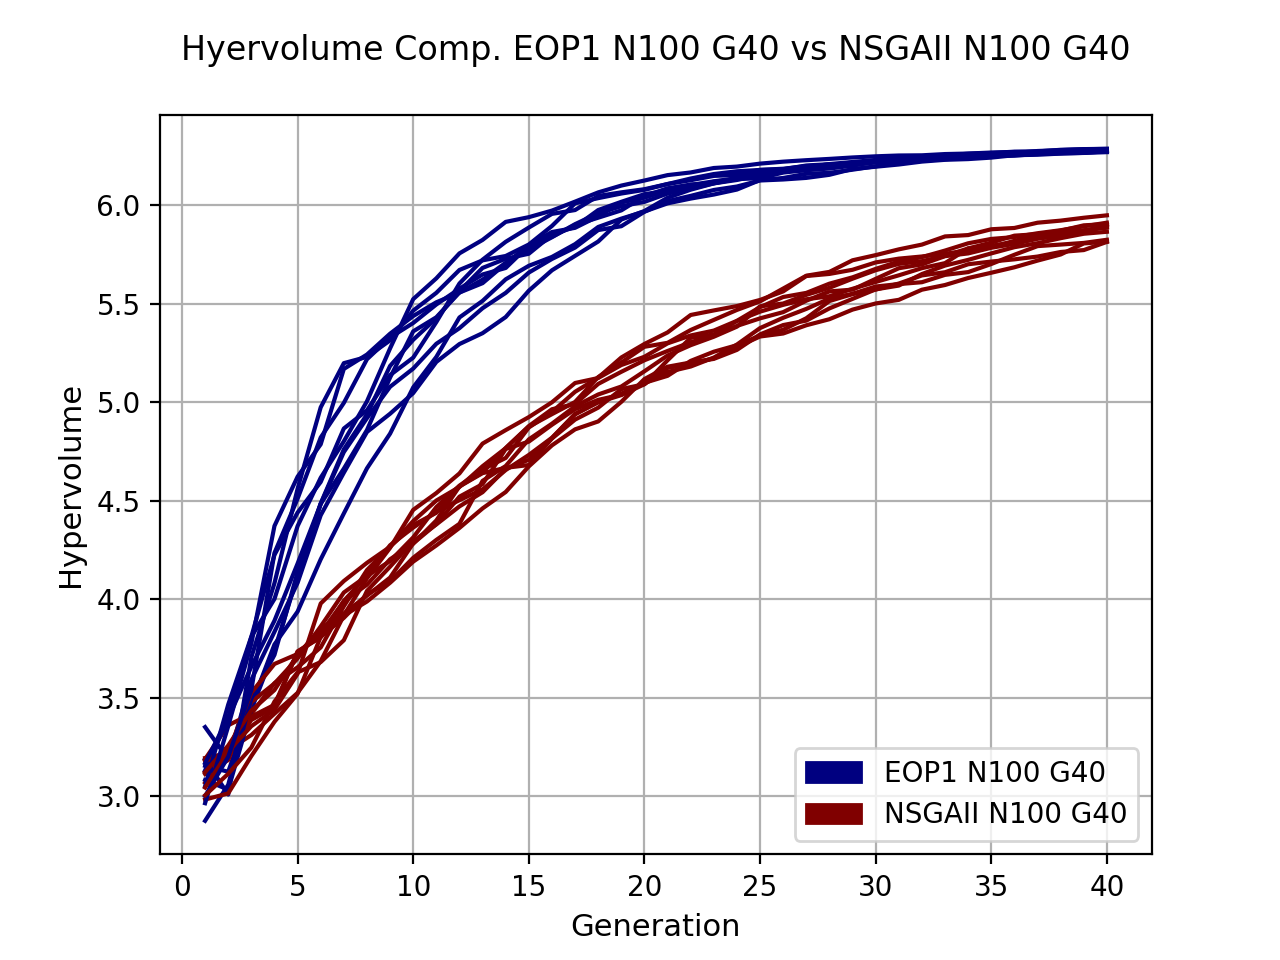
\includegraphics[scale=0.35]{../METRICS_PLOTS/Hypervol_COMP_EOP1N100G40_NSGAIIN100G40.png}
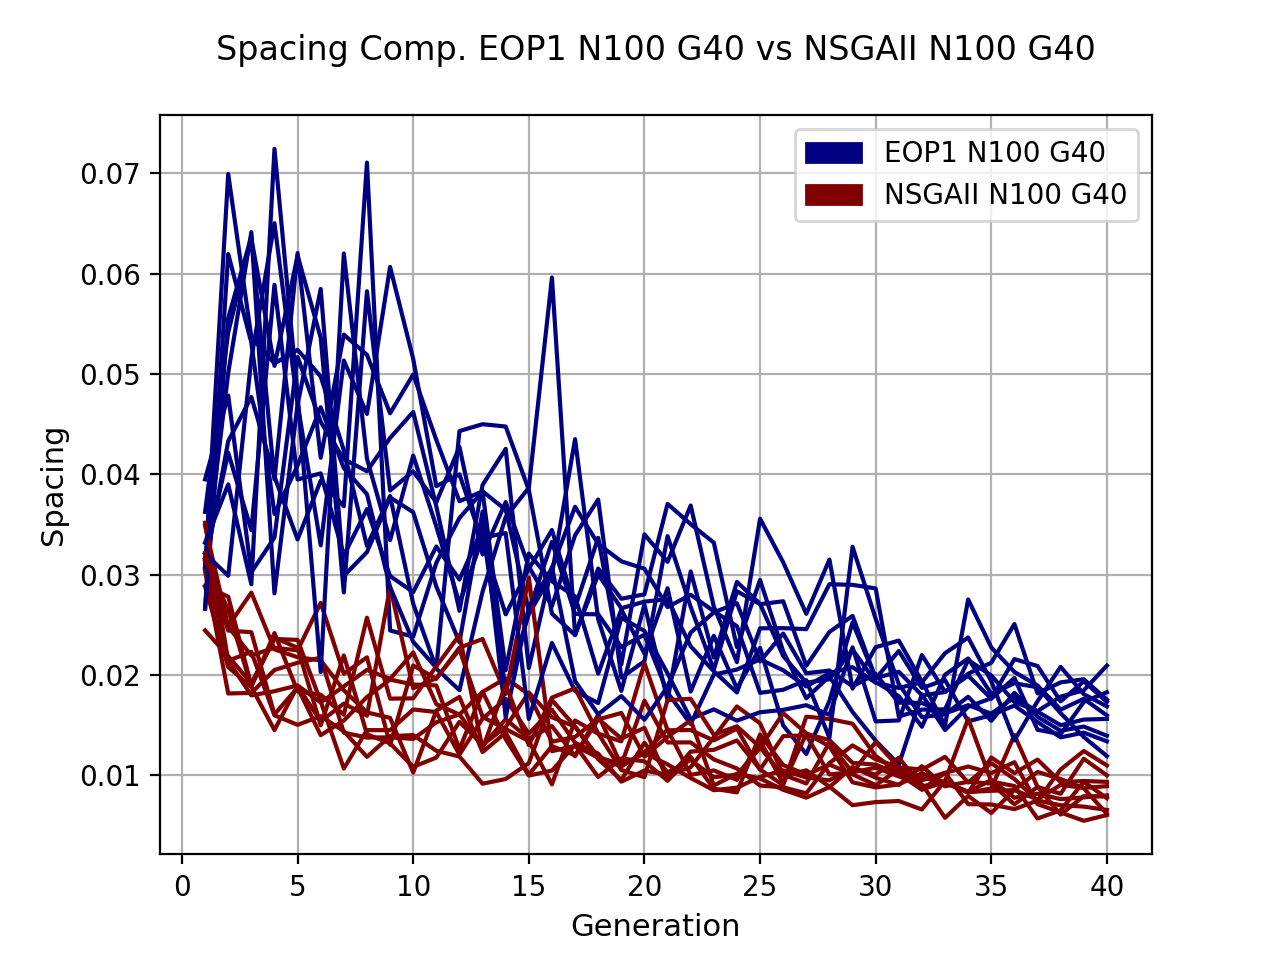
\includegraphics[scale=0.35]{../METRICS_PLOTS/Spacing_COMP_EOP1N100G40_NSGAIIN100G40.png}
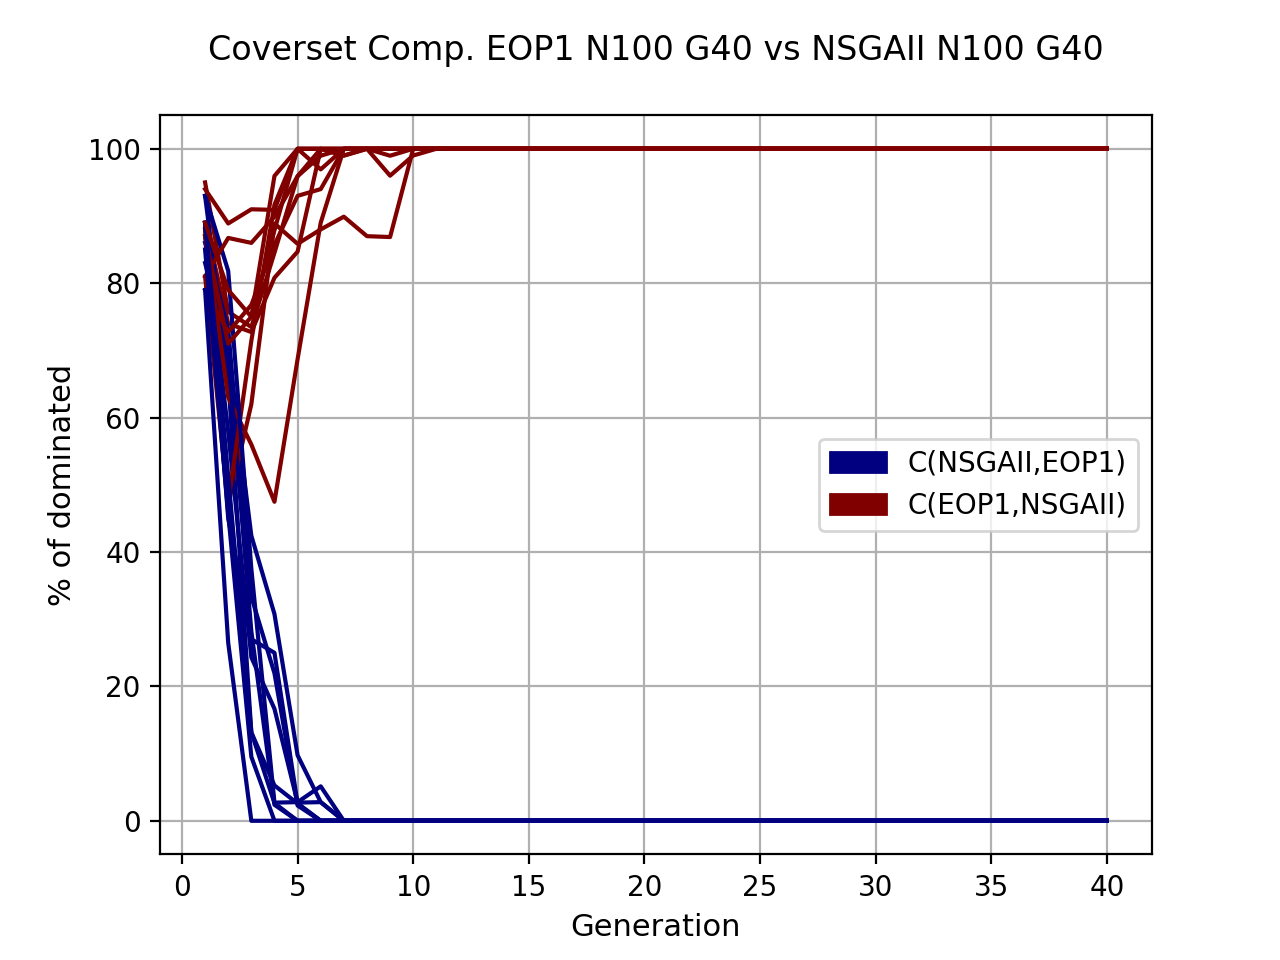
\includegraphics[scale=0.35]{../METRICS_PLOTS/CoverSet_COMP_EOP1N100G40_NSGAIIN100G40.png}\\
\caption{MOEA/D + EOP1. Comparación de métricas con NSGAII para 4000 EV.}
\label{fig:9}
\end{figure}



